% =============================================================================
% Master's Thesis (TFM) - Part II (extended version)
% "Quantum control for quantum information transfer mediated by
%  topological edge states"
% Template: REVTeX 4.2 (APS format)
%
% Changes from Part I:
%   - Abstract: removed inline journal citations
%   - Body: author names include initials throughout
%   - Fig. 9 caption: corrected panel description
%   - Fig. 11 left-panel title: fixed in Python source (now English)
%   - Fig. 12 table headers: fixed in Python source (now English)
%   - Section V.E last sentence: highlighted in bold
%   - NEW Section VIII: CTAP — dynamic control beyond the static Rabi regime
%   - Updated conclusions (Section IX)
% =============================================================================
\documentclass[
  reprint,
  amsmath,
  amssymb,
  aps,
  prb,
  floatfix,
  longbibliography,
]{revtex4-2}

\usepackage{graphicx}
\usepackage{dcolumn}
\usepackage{bm}
\usepackage{hyperref}
\usepackage{xcolor}
\usepackage{braket}
\usepackage{booktabs}
\usepackage{siunitx}
\usepackage{float}
\usepackage{tikz}
\usepackage{morefloats}
\usetikzlibrary{calc,decorations.pathreplacing}

\graphicspath{{figures/}}

% Custom commands
\newcommand{\hop}[1]{t_{#1}}
\newcommand{\ttr}{t_{\mathrm{tr}}}
\newcommand{\tprep}{t_{\mathrm{prep}}}
\newcommand{\Heff}{\mathcal{H}_{\mathrm{eff}}}
\newcommand{\JLS}{J_{\mathcal{LS}}}
\newcommand{\JSR}{J_{\mathcal{SR}}}
\newcommand{\ketL}{\ket{\mathcal{L}}}
\newcommand{\ketS}{\ket{\mathcal{S}}}
\newcommand{\ketR}{\ket{\mathcal{R}}}

\begin{document}

% ============================================================================
\title{Quantum control for quantum information transfer mediated by topological edge states}

\author{Miguel García-Mier García}
% \email{your.email@university.edu}
\affiliation{%
  MSc in Quantum Technologies, Universidad Internacional Men\'endez Pelayo, Spain
}

\date{May 2026}

\begin{abstract}
We study quantum state transfer in one-dimensional topological chains based on the
Su-Schrieffer-Heeger (SSH) model, comparing two distinct paradigms:
domain wall-mediated transfer and counterdiabatic (CD) driving.
First, we numerically reproduce a domain wall transfer protocol,
achieving fidelities $f > 0.999$ for symmetric two-domain configurations with
$L = 11$ sites. We investigate the effect of asymmetric domain wall placement,
demonstrating that the fidelity is constrained by the exponential
sensitivity of the effective couplings to the domain lengths---a limitation of
the static Rabi protocol rather than of topological protection itself.
We further explore shortcut-to-adiabaticity (STA) pulse protocols and find that
no pulse optimization can overcome the coupling asymmetry that governs the
transfer phase.
Second, we present an extensive analysis of a hybrid analog-digital protocol
for nonadiabatic edge-state transfer, where the SSH Hamiltonian is supplemented
with approximate counterdiabatic interactions derived from adiabatic gauge
potentials and optimized via variational quantum circuits.
Third, motivated by the CTAP (Coherent Tunnelling Adiabatic Passage) formalism,
we show analytically that the coupling asymmetry can be overcome by replacing the
static Rabi protocol with a dynamic counter-intuitive pulse sequence that
exploits the topological dark state of the effective three-level Hamiltonian.
We discuss extensions to two-domain wall systems, showing that the even-state
parity constraint imposes fundamental limitations on the standard CTAP scheme.
\end{abstract}

\maketitle

% ============================================================================
\section{Introduction}
\label{sec:intro}

Quantum state transfer---the coherent transport of quantum information between
distant nodes of a quantum network---is a fundamental primitive for quantum
computing and communication architectures~\cite{Bose2003, Christandl2004,
Nikolopoulos2014}. In solid-state platforms such as quantum dot arrays,
superconducting circuits, or cold-atom lattices, the transfer must contend with
disorder, decoherence, and the difficulty of precisely engineering long-range
couplings.

A promising approach exploits the \emph{topological protection} of edge states in
one-dimensional lattice models~\cite{Hasan2010, Asboth2016}. The
Su-Schrieffer-Heeger (SSH) model~\cite{SSH1979, SSH1980}---a paradigmatic
example of a symmetry-protected topological insulator in class BDI~\cite{Ryu2010}---supports
exponentially localized zero-energy edge states when the system is in the
topological phase. These states are robust against local perturbations that respect
the protecting chiral symmetry, making them attractive candidates as quantum
information carriers.

J.~Zurita, C.~E.~Creffield, and G.~Platero~\cite{Zurita2023} demonstrated that chains
comprising multiple SSH domains separated by \emph{topological domain walls}
can mediate fast, high-fidelity quantum transfer. The key mechanism is an
exponential speed-up arising from the multi-domain structure: by distributing
$N$ domain walls along the chain, the transfer time scales as
$(w/v)^{\ell/2}$ per domain (where $\ell$ is the domain length and $v/w$ the
hopping ratio) rather than $(w/v)^{L/2}$ for the entire chain. This exponential
compression of the transfer time, combined with the topological robustness of
the boundary states, provides a powerful paradigm for quantum information
transport.

In this work, we present a study on topological
quantum transfer in SSH chains. We focus on two-domain ($N = 2$) SSH chains and address three
questions:
\begin{enumerate}
  \item Can the transfer protocol of Ref.~\cite{Zurita2023} be faithfully
    reproduced numerically, and what are the optimal parameters?
  \item How does the transfer fidelity degrade when the domain wall is displaced
    from the chain center, breaking the symmetry between the two domains?
  \item Can shortcut-to-adiabaticity (STA) pulse
    protocols~\cite{Demirplak2003, Berry2009, GueryOdelin2019} improve the
    transfer performance, particularly in asymmetric configurations?
\end{enumerate}

Additionally, we provide a comprehensive analysis of an alternative approach:
the hybrid analog-digital protocol recently proposed by
S.~V.~Romero, X.~Chen, G.~Platero, and Y.~Ban~\cite{Romero2024}, where nonadiabatic transfer is
achieved through counterdiabatic (CD) driving rather than topological domain
walls. We compare both paradigms in terms of their physical mechanisms,
scalability, and robustness.

Finally, motivated by the CTAP framework of
A.~D.~Greentree, J.~H.~Cole, A.~R.~Hamilton, and L.~C.~L.~Hollenberg~\cite{Greentree2004},
we show how the limitations of the static Rabi protocol in asymmetric
configurations can be overcome by means of a dynamic counter-intuitive pulse
sequence that exploits the topological dark state of the effective three-level
Hamiltonian.

The remainder of this document is organized as follows.
Section~\ref{sec:model} introduces the SSH model, its topological properties,
and the domain wall construction. Section~\ref{sec:transfer} describes the
transfer protocol and presents our reproduction of the main results
of Ref.~\cite{Zurita2023}. Section~\ref{sec:asymmetric} analyzes the effect of
asymmetric domain wall placement. Section~\ref{sec:sta} investigates
STA pulse protocols.
Section~\ref{sec:cd_protocol} presents a detailed exposition of the hybrid
analog-digital counterdiabatic protocol. Section~\ref{sec:comparison} provides
a systematic comparison of the domain wall and counterdiabatic approaches.
Section~\ref{sec:ctap} introduces the CTAP framework as a route beyond the
static Rabi limitation, analyzes the topological dark state, and discusses
extensions to two-domain wall systems.
Section~\ref{sec:conclusions} summarizes our findings and outlines future
directions.

% ============================================================================
\section{The SSH model and domain walls}
\label{sec:model}

% --- 2.1 Hamiltonian ---
\subsection{The Su-Schrieffer-Heeger Hamiltonian}
\label{sec:ssh}

The SSH model describes a one-dimensional tight-binding chain with alternating
hopping amplitudes $v$ (intracell) and $w$ (intercell)~\cite{SSH1979,SSH1980}.
For a chain of $L$ sites labeled $j = 0, 1, \ldots, L-1$, the Hamiltonian reads
\begin{equation}
  \mathcal{H} = -\sum_{j=0}^{L-2} t_j
  \bigl(\ket{j}\bra{j+1} + \ket{j+1}\bra{j}\bigr),
  \label{eq:ssh_ham}
\end{equation}
where
\begin{equation}
  t_j =
  \begin{cases}
    v & \text{if } j \text{ is even (intracell)}, \\
    w & \text{if } j \text{ is odd (intercell)}.
  \end{cases}
  \label{eq:hoppings}
\end{equation}
The unit cell contains two sites---sublattice $a$ (even sites) and sublattice $b$
(odd sites). In the thermodynamic limit ($L \to \infty$), the Bloch Hamiltonian
in momentum space is $\mathcal{H}(k) = \bm{d}(k) \cdot \bm{\sigma}$, where
$\bm{\sigma} = (\sigma_x, \sigma_y)$ and the winding of $\bm{d}(k)$ around the
origin classifies the topological phases.

% --- 2.2 Spectrum and gap ---
\subsection{Energy spectrum and topological transition}
\label{sec:spectrum}

The bulk dispersion relation is
\begin{equation}
  E(k) = \pm\sqrt{v^2 + w^2 + 2vw\cos k},
  \label{eq:dispersion}
\end{equation}
yielding a spectral gap
\begin{equation}
  \Delta = 2|w - v|
  \label{eq:gap}
\end{equation}
that closes at $v = w$, signaling the topological phase transition. For $v < w$
the system is in the \emph{topological phase} with winding number $\nu = 1$,
while for $v > w$ it is in the \emph{trivial phase} with $\nu = 0$~\cite{Zak1989, Asboth2016}.

Figure~\ref{fig:spectrum} shows the energy spectrum of a finite SSH chain
($L = 10$) as a function of $v/w$. The gap closes linearly at the critical point
$v = w$. For a chain with an odd number of sites ($L = 11$), a zero-energy edge
state appears in the topological phase, manifesting the bulk-boundary
correspondence~\cite{Prodan2016}.

\begin{figure*}[t]
  \centering
  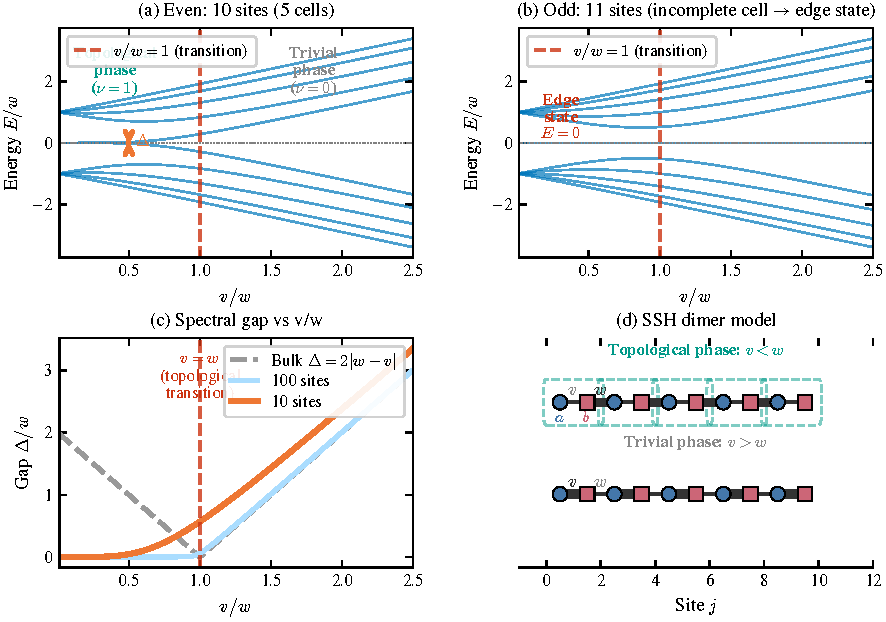
\includegraphics[width=\textwidth]{fig1_dimer_spectrum.pdf}
  \caption{Energy spectrum of the SSH dimer chain as a function of the hopping
  ratio $v/w$. \textbf{Left:} Even chain ($L = 10$). The bulk gap
  $\Delta = 2|w - v|$ closes at $v = w$. \textbf{Right:} Odd chain ($L = 11$).
  A zero-energy state (red) appears in the topological phase ($v/w < 1$),
  localized at the boundary.}
  \label{fig:spectrum}
\end{figure*}

% --- 2.3 Topology ---
\subsection{Topological invariant}
\label{sec:topology}

The topological classification of the SSH model is captured by the
\emph{winding number}
\begin{equation}
  \nu = \frac{1}{2\pi} \oint dk \; \frac{d}{dk}
  \arg\bigl[d_x(k) + i\, d_y(k)\bigr],
  \label{eq:winding}
\end{equation}
where $d_x(k) = v + w\cos k$ and $d_y(k) = w\sin k$. The winding number counts
how many times the vector $\bm{d}(k)$ encircles the origin as $k$ traverses the
Brillouin zone. For the SSH model:
\begin{itemize}
  \item $v < w$: $\bm{d}(k)$ encircles the origin $\Rightarrow$ $\nu = 1$ (topological),
  \item $v > w$: $\bm{d}(k)$ does not encircle the origin $\Rightarrow$ $\nu = 0$ (trivial).
\end{itemize}
The winding number is quantized and can only change when the gap closes ($v = w$),
reflecting its topological nature. By the bulk-boundary correspondence, a chain
with $\nu = 1$ hosts one protected zero-energy state per boundary.

% --- 2.4 Domain walls ---
\subsection{Domain walls and protected states}
\label{sec:dw}

A \emph{domain wall} (DW) is created at the interface between two SSH domains
with different dimerization patterns. Consider a chain of total length $L$ composed
of two domains meeting at site $j_{\mathrm{DW}}$:
\begin{itemize}
  \item \textbf{Domain 1} ($j < j_{\mathrm{DW}}$): standard SSH hopping pattern $(v, w, v, w, \ldots)$,
  \item \textbf{Domain 2} ($j \geq j_{\mathrm{DW}}$): the pattern restarts as $(v, w, v, w, \ldots)$.
\end{itemize}
When $j_{\mathrm{DW}}$ is at an \emph{odd} site, the bond at the interface involves two
consecutive $v$-bonds (a $vv$ defect), which constitutes a topological domain wall.
This is because the dimerization pattern on each side of the interface is conjugate:
if the left domain is in the topological phase, the right domain effectively
presents the reversed pattern.

For a chain with $N = 2$ domains (one domain wall), the system hosts three
topologically protected states near $E = 0$ (Fig.~\ref{fig:dw_states}):
\begin{align}
  \ketL &\propto \sum_{n=0}^{\ell_1/2}(-r)^n \ket{2n},
  \label{eq:ketL} \\
  \ketS &\propto \ket{j_{\mathrm{DW}}} + \sum_{n=1}^{\ell_1/2}(-r)^n
  \ket{j_{\mathrm{DW}} - 2n}
  \nonumber \\
  &\quad + \sum_{n=1}^{\ell_2/2}(-r)^n \ket{j_{\mathrm{DW}} + 2n},
  \label{eq:ketS} \\
  \ketR &\propto \sum_{n=0}^{\ell_2/2}(-r)^n \ket{L - 1 - 2n},
  \label{eq:ketR}
\end{align}
where $r = v/w$ is the decay ratio, and $\ell_1$, $\ell_2$ are the lengths
(number of bonds) of the left and right domains, respectively. Each state
resides on a single sublattice and decays exponentially away from its localization
center with characteristic length $\xi = -1/\ln r$.

\begin{figure*}[t]
  \centering
  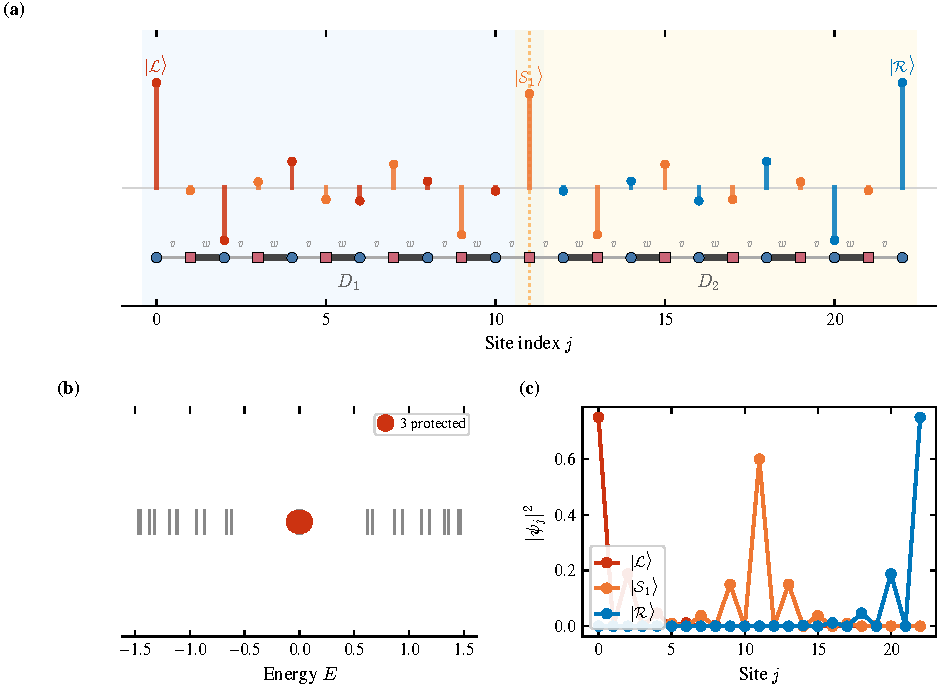
\includegraphics[width=\textwidth]{fig2_domain_wall_states.pdf}
  \caption{Topologically protected states in a two-domain SSH chain ($L = 23$,
  $N = 2$, $\ell = 10$, $v = 0.5$, $w = 1.0$). The three states $\ketL$,
  $\ketS$, and $\ketR$ are localized at the left edge, the domain wall, and the
  right edge, respectively. Sublattice polarization (alternating signs) is
  clearly visible.}
  \label{fig:dw_states}
\end{figure*}

% --- 2.5 Effective Hamiltonian ---
\subsection{Effective low-energy Hamiltonian}
\label{sec:heff}

The three protected states span an effective low-energy subspace described by
\begin{equation}
  \Heff = \JLS \ketS\!\bra{\mathcal{L}} + \JSR \ketR\!\bra{\mathcal{S}} + \text{H.c.},
  \label{eq:heff}
\end{equation}
which has the structure of a three-site tight-binding chain. The effective couplings
$\JLS$ and $\JSR$ depend on the overlap of adjacent protected states through the
SSH bulk. From the analytical expressions [Eqs.~(\ref{eq:ketL})--(\ref{eq:ketR})],
these couplings scale as~\cite{Zurita2023}
\begin{equation}
  J \sim v \cdot \mathcal{M}_i \cdot \mathcal{M}_j \cdot
  \left(\frac{v}{w}\right)^{\!\ell/2},
  \label{eq:coupling_scaling}
\end{equation}
where $\ell$ is the domain length separating the two states, and the normalization
constants are
\begin{equation}
  \mathcal{M}_{\mathcal{L}} = \mathcal{M}_{\mathcal{R}} =
  \sqrt{\frac{w^2}{v^2} - 1},
  \quad
  \mathcal{M}_{\mathcal{S}} = \sqrt{\frac{w^2 - v^2}{w^2 + v^2}}.
  \label{eq:normalization}
\end{equation}

\emph{Crucially}, the exponential dependence of $J$ on $\ell$ implies that even
a small asymmetry $\ell_1 \neq \ell_2$ leads to vastly different effective
couplings:
\begin{equation}
  \frac{\JLS}{\JSR} \sim
  \left(\frac{w}{v}\right)^{\!(\ell_2 - \ell_1)/2}.
  \label{eq:coupling_ratio}
\end{equation}
For our parameters $w = 2v$, a difference $|\ell_1 - \ell_2| = 2$ already produces
a coupling ratio of~4, while $|\ell_1 - \ell_2| = 8$ yields a ratio of~$2^4 = 16$.

% ============================================================================
\section{Transfer protocol}
\label{sec:transfer}

\subsection{Adiabatic preparation and readout}
\label{sec:protocol}

The transfer protocol proposed by J.~Zurita, C.~E.~Creffield, and G.~Platero~\cite{Zurita2023}
consists of three phases:
\begin{enumerate}
  \item \textbf{Preparation} ($0 \leq t < \tprep$): The intracell hopping
    is ramped from $v = 0$ (fully dimerized) to $v = v_{\mathrm{tr}}$
    following a smooth pulse shape. This adiabatically maps the initial
    localized state $\ket{0}$ onto the protected boundary state $\ketL$.
  \item \textbf{Transfer} ($\tprep \leq t < \ttr - \tprep$): The hopping
    is held constant at $v = v_{\mathrm{tr}}$. The effective couplings
    $\JLS$, $\JSR$ drive Rabi-like oscillations in the protected subspace,
    transferring population from $\ketL$ to $\ketR$ via $\ketS$.
  \item \textbf{Readout} ($\ttr - \tprep \leq t \leq \ttr$): The hopping
    is ramped back to $v = 0$, adiabatically mapping $\ketR$ back onto the
    localized state $\ket{L-1}$.
\end{enumerate}

The standard pulse shape (Eq.~(11) of Ref.~\cite{Zurita2023}) is
\begin{equation}
  v(t) =
  \begin{cases}
    v_{\mathrm{tr}} \sin^2\!\bigl(\Omega t\bigr) & 0 \leq t < \tprep, \\
    v_{\mathrm{tr}} & \tprep \leq t < \ttr - \tprep, \\
    v_{\mathrm{tr}} \sin^2\!\bigl(\Omega(t - \ttr)\bigr) & \ttr - \tprep \leq t \leq \ttr,
  \end{cases}
  \label{eq:pulse}
\end{equation}
with $\Omega = \pi/(2\tprep)$. The $\sin^2$ ramp is chosen for its smoothness:
both $v(t)$ and $\dot{v}(t)$ vanish at $t = 0$ and $t = \tprep$, minimizing
diabatic transitions to bulk states. The adiabatic condition requires
$\tprep \gg \tau = 2/\Delta$, where $\Delta$ is the instantaneous spectral gap.

The transfer fidelity is defined as the occupation probability of the target
site at the end of the protocol:
\begin{equation}
  f = \bigl|\braket{L-1|\psi(\ttr)}\bigr|^2.
  \label{eq:fidelity}
\end{equation}

\subsection{Transfer time}
\label{sec:transfer_time}

For a symmetric two-domain chain ($\ell_1 = \ell_2 = \ell$), the effective
Hamiltonian~(\ref{eq:heff}) has equal couplings $\JLS = \JSR \equiv J$.
The time for complete population transfer from $\ketL$ to $\ketR$ via the
intermediate state $\ketS$ in a uniform three-site chain is
\begin{equation}
  \ttr^{\mathrm{eff}} = \frac{\pi}{\sqrt{2}\, J},
  \label{eq:ttr_sym}
\end{equation}
which, using Eq.~(\ref{eq:coupling_scaling}), scales exponentially with the
domain length:
\begin{equation}
  \ttr \sim \frac{\pi(w^2 + v^2)}{2(w^2 - v^2)}
  \left(\frac{w}{v}\right)^{\!\ell/2 + 1}.
  \label{eq:ttr_analytical}
\end{equation}

\subsection{Numerical results: reproducing Ref.~\cite{Zurita2023}}
\label{sec:results_symmetric}

We simulate the full time-dependent Schr\"odinger equation for a chain of
$L = 11$ sites ($N = 2$ domains, $\ell = 4$) with $w = 1.0$, $v_{\mathrm{tr}} = 0.5$,
and $\tprep = 15$. The time evolution is performed via exact exponentiation of
the Hamiltonian at each time step $\Delta t = 0.5$.

Figure~\ref{fig:transfer} shows the transfer dynamics for $\ttr = 45.0$.
The initial state $\ket{0}$ is clearly seen to evolve through the three
protected states: population flows from the left edge to the domain wall and
then to the right edge, achieving a final fidelity $f = 0.999$.

\begin{figure}[t]
  \centering
  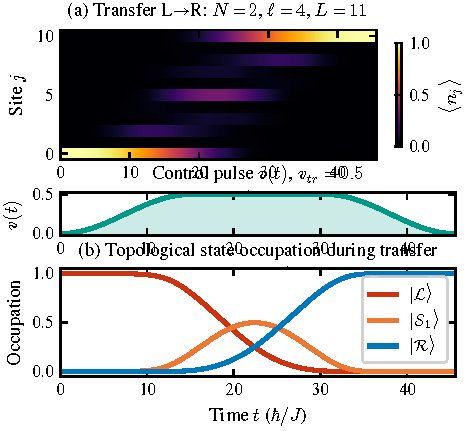
\includegraphics[width=\columnwidth]{fig3_transfer_protocol.pdf}
  \caption{Transfer protocol dynamics for the symmetric two-domain SSH chain
  ($L = 11$, $\ell = 4$, $v_{\mathrm{tr}} = 0.5$, $w = 1.0$, $\tprep = 15$,
  $\ttr = 45$). Population is transferred from site $0$ to site $10$ via the
  topologically protected subspace, with final fidelity $f = 0.999$.}
  \label{fig:transfer}
\end{figure}

Figure~\ref{fig:fidelity_scan} presents the fidelity as a function of
$\ttr$, showing Rabi-like oscillations with the first maximum at
$\ttr \approx 45$, in excellent agreement with the theoretical prediction
$\ttr \approx 45.6$ from Eq.~(\ref{eq:ttr_analytical}) and the value
reported in Ref.~\cite{Zurita2023}. The peak fidelity $f = 0.999$ exceeds
the threshold $f_0 = 0.995$ commonly cited for fault-tolerant quantum error
correction~\cite{Knill2005}.

\begin{figure}[t]
  \centering
  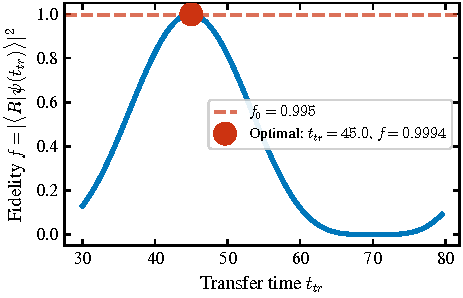
\includegraphics[width=\columnwidth]{fig4_fidelity_scan.pdf}
  \caption{Transfer fidelity as a function of the total protocol time $\ttr$
  for the symmetric chain ($L = 11$, $\ell = 4$). The first maximum occurs at
  $\ttr \approx 45$ with $f = 0.999$, consistent with Ref.~\cite{Zurita2023}.
  Subsequent oscillations arise from the Rabi dynamics of the effective
  three-site chain.}
  \label{fig:fidelity_scan}
\end{figure}

% ============================================================================
\section{Asymmetric domain wall placement}
\label{sec:asymmetric}

\subsection{Motivation}
\label{sec:asym_motivation}

In practice, fabrication imperfections may shift the domain wall away from the
ideal center of the chain. Furthermore, for chains of certain lengths, it is
geometrically impossible to place the domain wall exactly at the center. The
domain wall position $j_{\mathrm{DW}}$ must be at an \emph{odd-index} site for
the $vv$-bond defect to occur; thus, only chains with $L = 4k + 3$ (i.e.,
$L = 11, 15, 19, 23, \ldots$) admit a perfectly centered domain wall with
$\ell_1 = \ell_2$.

We study a chain of $L = 21$ sites (10 complete unit cells plus one boundary
site), varying the domain wall position among three representative odd sites:
\begin{itemize}
  \item $j_{\mathrm{DW}} = 11$ (quasi-center): $\ell_1 = 11$, $\ell_2 = 9$,
  \item $j_{\mathrm{DW}} = 7$ (one-third): $\ell_1 = 7$, $\ell_2 = 13$,
  \item $j_{\mathrm{DW}} = 5$ (one-quarter): $\ell_1 = 5$, $\ell_2 = 15$.
\end{itemize}

\subsection{Protected states in asymmetric configurations}
\label{sec:asym_states}

Regardless of the domain wall position, the system always hosts three protected
states near $E = 0$, given by Eqs.~(\ref{eq:ketL})--(\ref{eq:ketR}) with
$\ell_1 \neq \ell_2$. We verify this numerically by diagonalizing the full
Hamiltonian and comparing the three eigenstates closest to $E = 0$ with the
analytical predictions. Table~\ref{tab:asym_states} summarizes the results.

\begin{table}[b]
  \caption{Protected states for the asymmetric domain wall configurations in an
  $L = 21$ chain ($v = 0.5$, $w = 1.0$). The subspace overlap is computed as
  the singular values of the overlap matrix between analytical and numerical
  eigenstates.}
  \label{tab:asym_states}
  \begin{ruledtabular}
  \begin{tabular}{ccccc}
    $j_{\mathrm{DW}}$ & $\ell_1 + \ell_2$ & $E_{\pm}$ &
    \textrm{Min.~overlap} & $\JLS/\JSR$ \\
    \colrule
    11 & $11 + 9$  & $\pm 0.024$ & 0.9998 & 0.50 \\
    7  & $7 + 13$  & $\pm 0.043$ & 0.9994 & 8.0  \\
    5  & $5 + 15$  & $\pm 0.086$ & 0.9978 & 32.0 \\
  \end{tabular}
  \end{ruledtabular}
\end{table}

Figure~\ref{fig:asym_states} illustrates how the spatial profiles of the
protected states change with the domain wall position. As the wall moves toward
the left edge, $\ketL$ becomes increasingly compressed into a shorter domain
(fewer sites available for its exponential tail), while $\ketR$ extends over
a longer domain. The state $\ketS$ develops an asymmetric envelope, decaying
faster into the shorter domain.

\begin{figure*}[t]
  \centering
  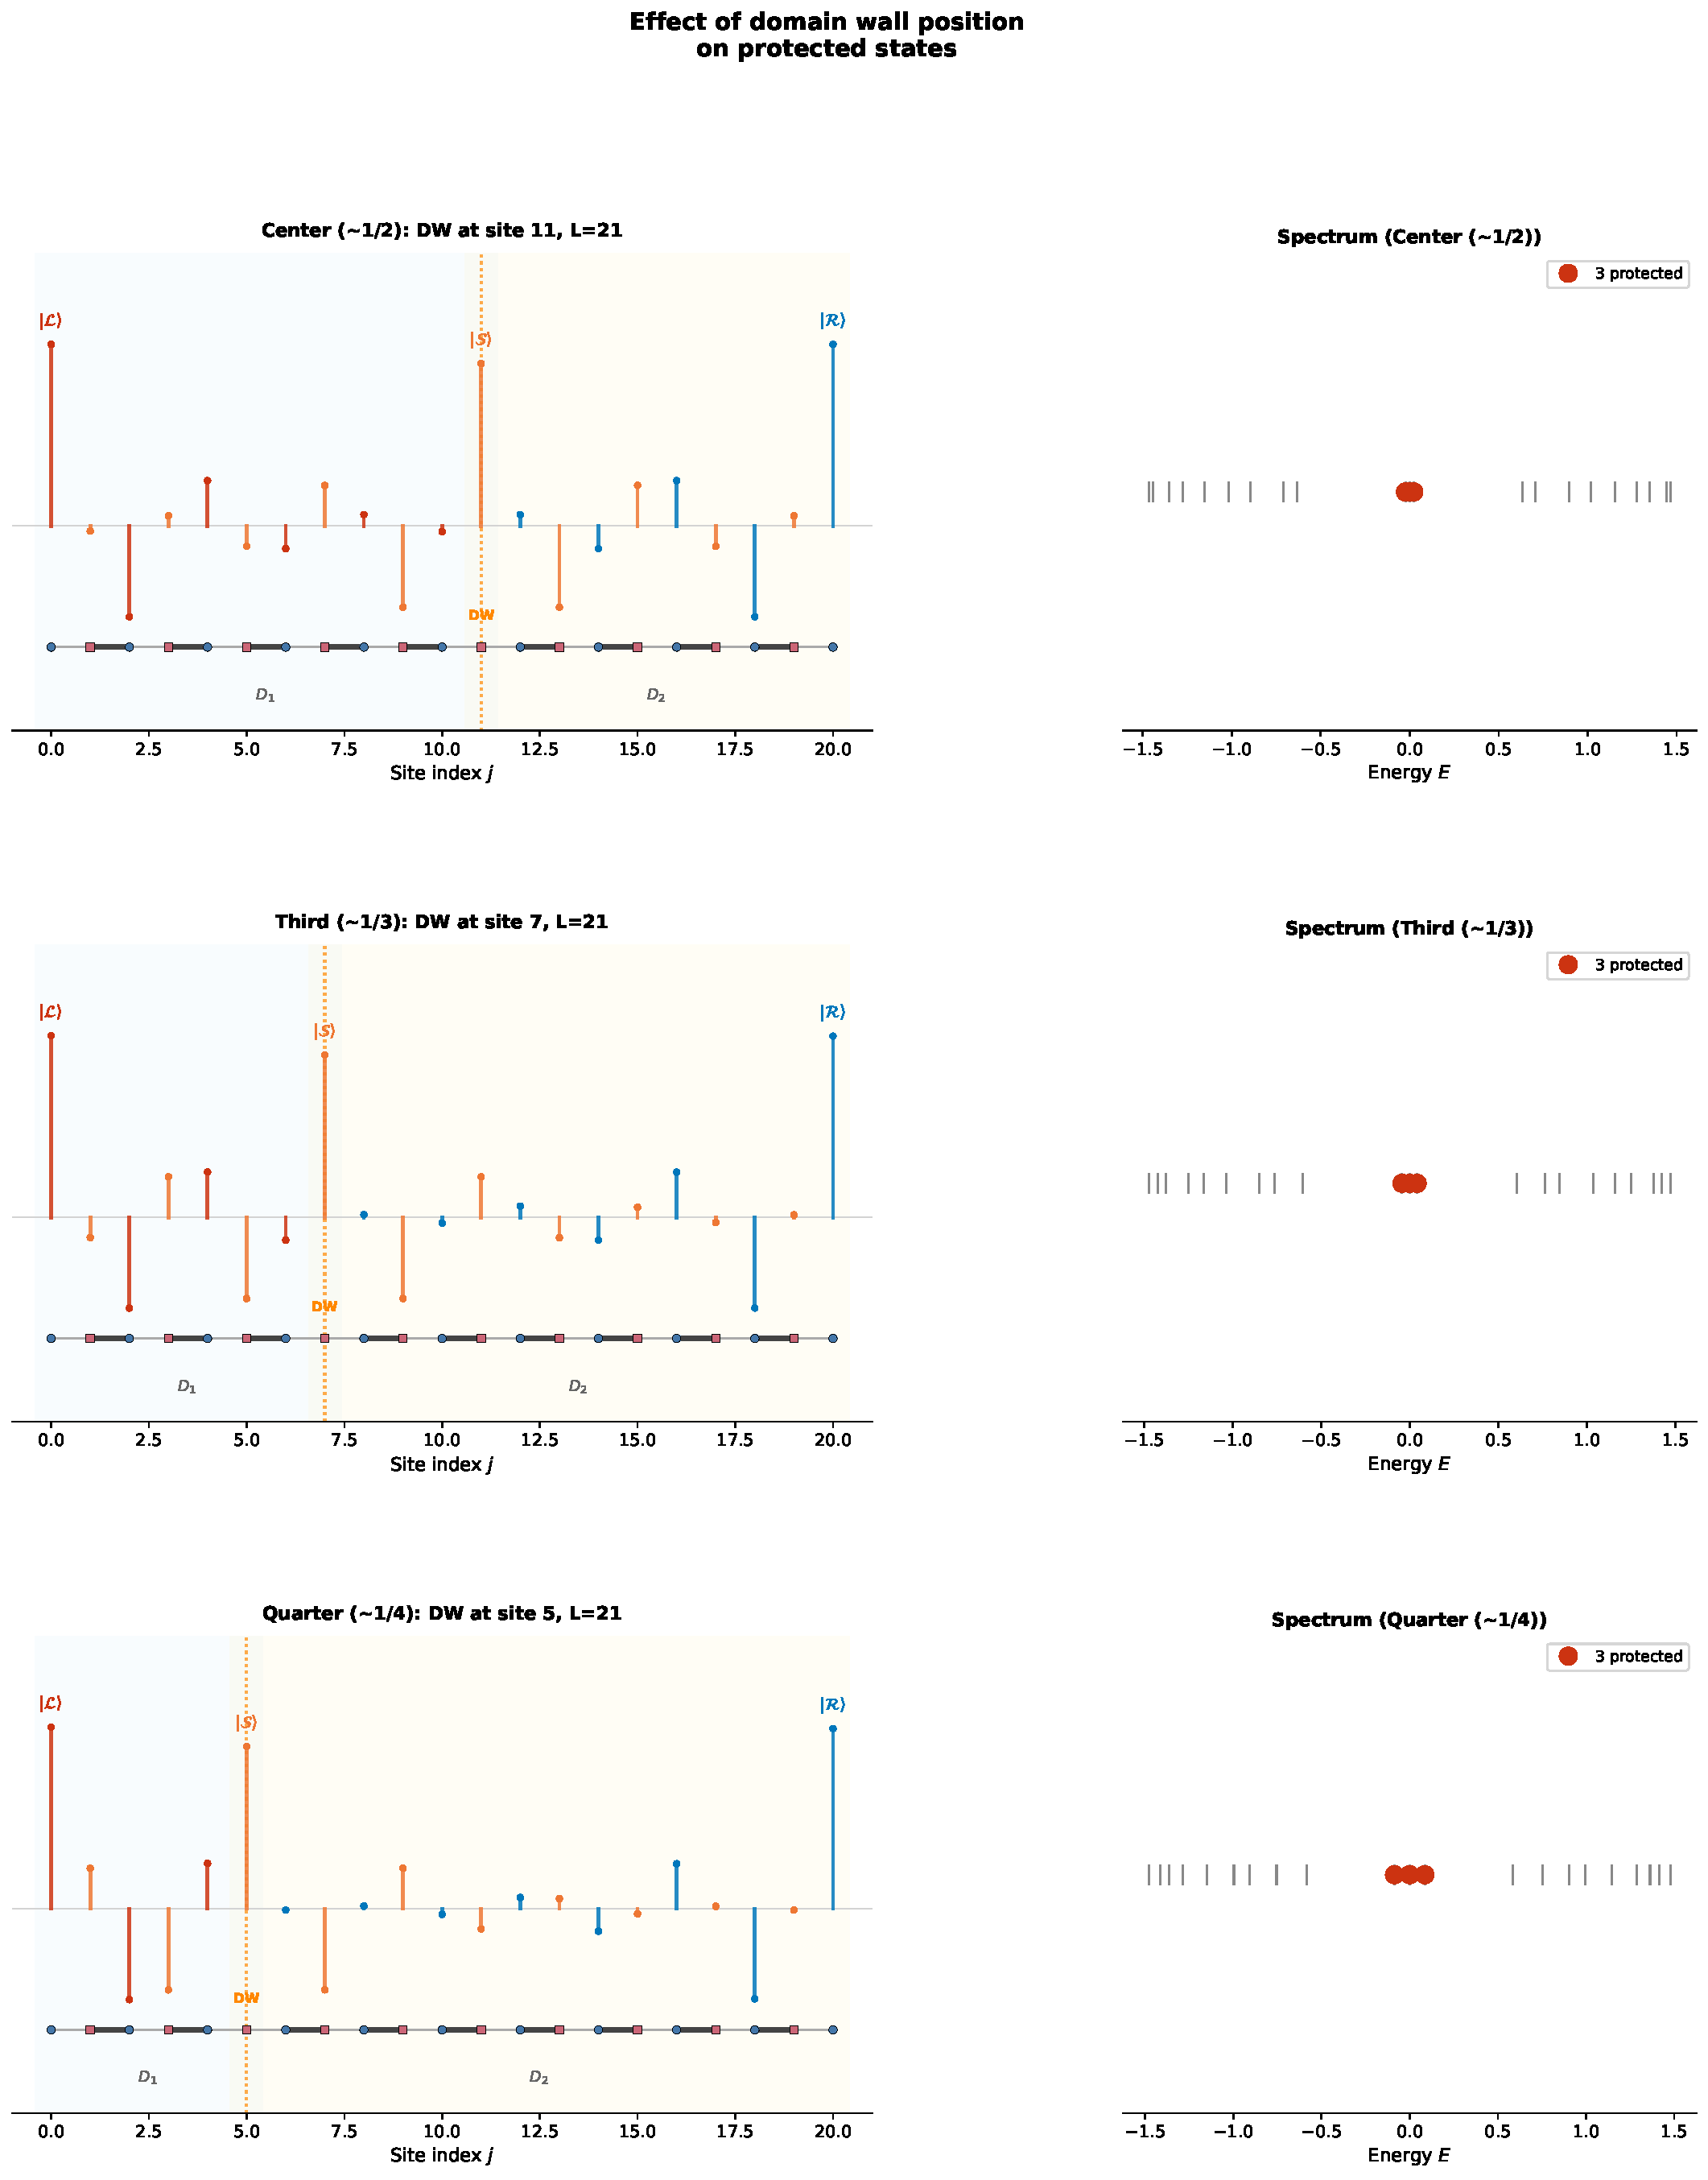
\includegraphics[width=\textwidth]{fig5_asymmetric_wall_states.pdf}
  \caption{Spatial profiles of the three protected states for different domain
  wall positions in an $L = 21$ chain. Top to bottom: $j_{\mathrm{DW}} = 11$
  (quasi-center), $j_{\mathrm{DW}} = 7$ (one-third), $j_{\mathrm{DW}} = 5$
  (one-quarter). The exponential localization and sublattice polarization are
  preserved in all cases.}
  \label{fig:asym_states}
\end{figure*}

\subsection{Effective couplings and the asymmetry mechanism}
\label{sec:asym_couplings}

The effective couplings $\JLS$ and $\JSR$ are computed numerically by
projecting the full Hamiltonian onto the protected subspace. The results
(Fig.~\ref{fig:coupling_asymmetry}) confirm the exponential scaling
predicted by Eq.~(\ref{eq:coupling_ratio}):

\begin{table}[b]
  \caption{Effective couplings for the three domain wall positions ($L = 21$,
  $v = 0.5$, $w = 1.0$).}
  \label{tab:couplings}
  \begin{ruledtabular}
  \begin{tabular}{ccccl}
    $j_{\mathrm{DW}}$ & $\JLS$ & $\JSR$ & Ratio & Predicted ratio \\
    \colrule
    11 & 0.0148 & 0.0296 & 0.50 & $(v/w)^1 = 0.50$ \\
    7  & 0.0593 & 0.0074 & 8.0  & $(w/v)^3 = 8.0$ \\
    5  & 0.1186 & 0.0037 & 32.0 & $(w/v)^5 = 32.0$ \\
  \end{tabular}
  \end{ruledtabular}
\end{table}

\begin{figure*}[t]
  \centering
  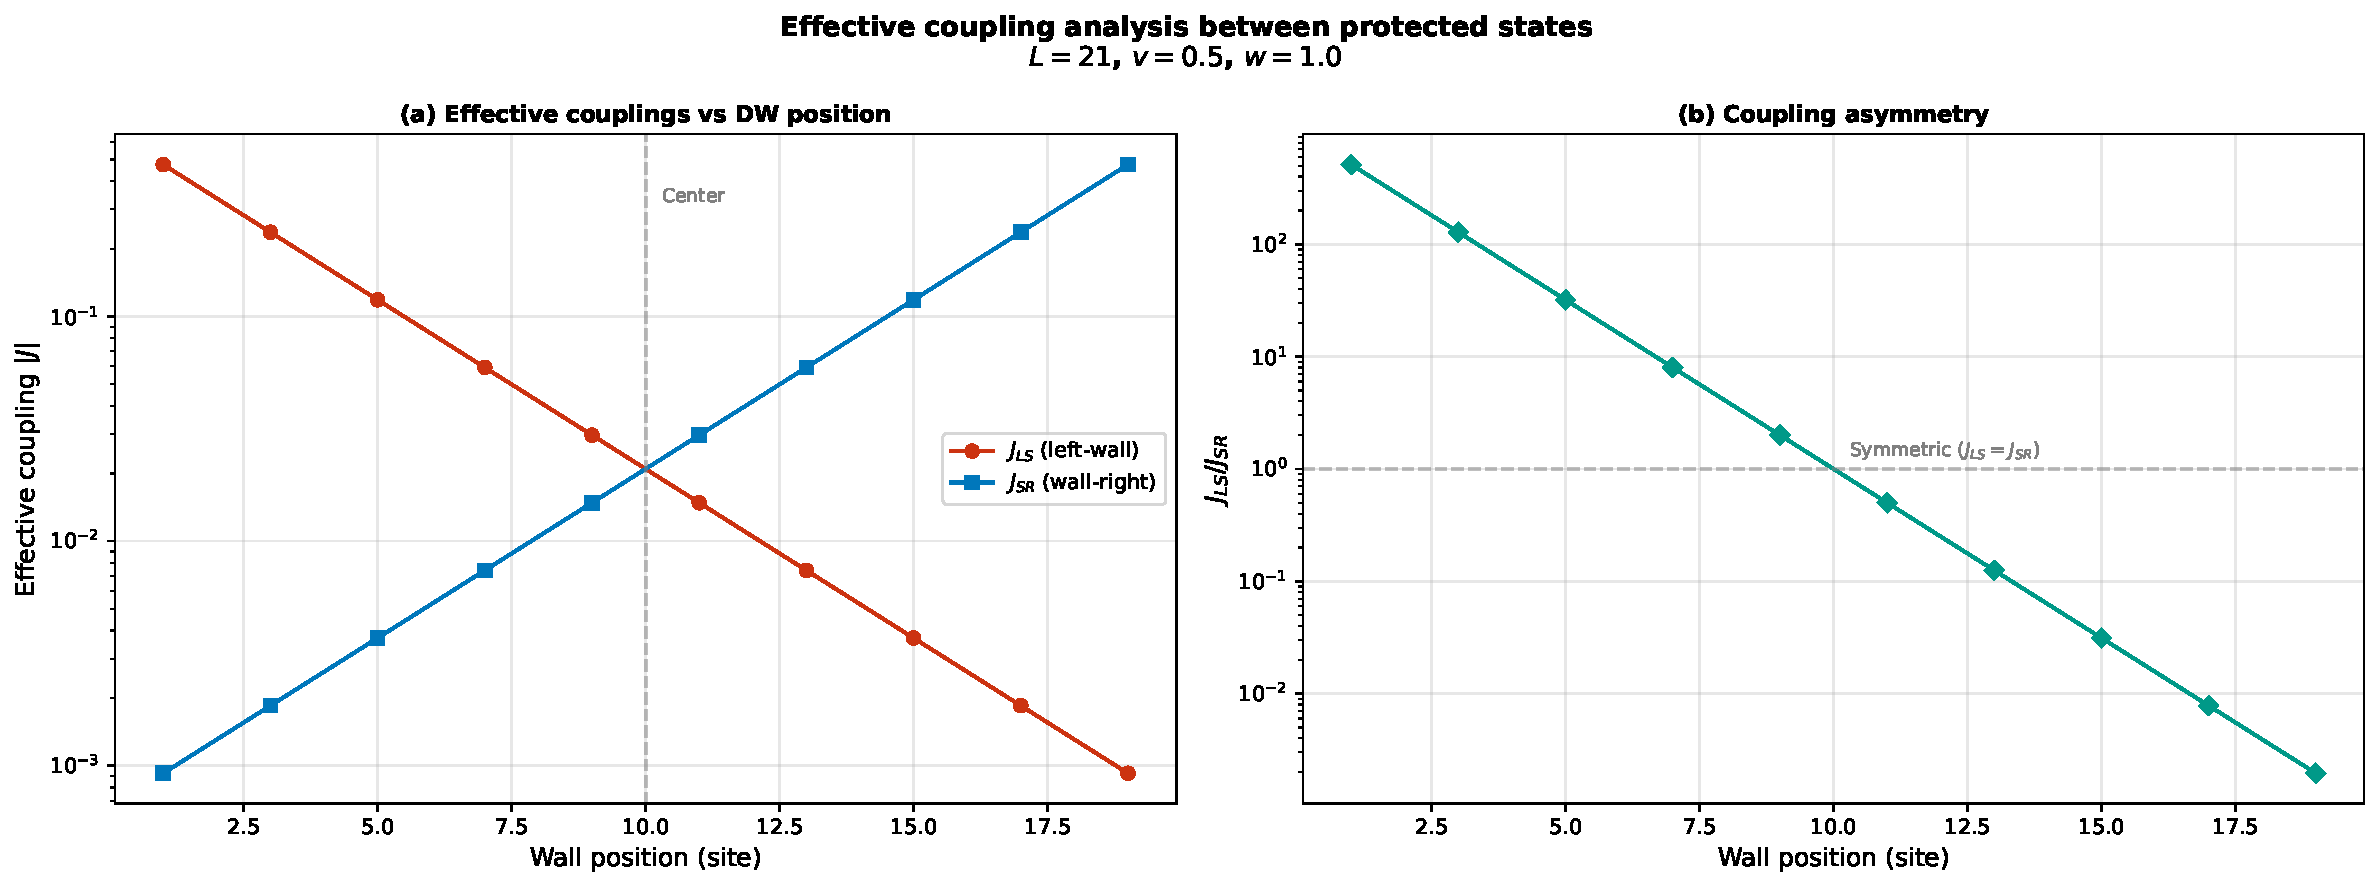
\includegraphics[width=\textwidth]{fig8_effective_coupling.pdf}
  \caption{Effective couplings $\JLS$ (left--soliton) and $\JSR$
  (soliton--right) as a function of the domain wall position for $L = 21$.
  The coupling asymmetry grows exponentially with the displacement from the
  chain center, consistent with Eq.~(\ref{eq:coupling_ratio}).}
  \label{fig:coupling_asymmetry}
\end{figure*}

The coupling asymmetry has a direct and dramatic consequence for the transfer
fidelity. In a three-site chain with unequal hoppings $J_1 \neq J_2$, the
maximum achievable population transfer from site 1 to site 3 is bounded
by~\cite{Christandl2004}
\begin{equation}
  f_{\max} = \frac{4 J_1^2 J_2^2}{(J_1^2 + J_2^2)^2},
  \label{eq:fmax}
\end{equation}
which equals unity only when $J_1 = J_2$ and decreases rapidly with the
coupling ratio. For our quasi-centered case ($\JLS/\JSR = 0.5$):
$f_{\max} = 4 \times 0.25/(1.25)^2 = 16/25 = 0.64$.

\subsection{Transfer fidelity in asymmetric chains}
\label{sec:asym_fidelity}

Figure~\ref{fig:asym_transfer} shows the transfer dynamics for the three
asymmetric configurations, using the standard $\sin^2$ pulse with $\tprep = 15$.
Table~\ref{tab:asym_fidelity} reports the optimal fidelities obtained from a
scan over $\ttr \in [30, 600]$.

\begin{table}[b]
  \caption{Optimal transfer fidelity for asymmetric domain wall positions
  ($L = 21$, standard $\sin^2$ pulse).}
  \label{tab:asym_fidelity}
  \begin{ruledtabular}
  \begin{tabular}{cccc}
    $j_{\mathrm{DW}}$ & $\ell_1 + \ell_2$ &
    $\ttr^{\mathrm{opt}}$ & $f_{\max}$ \\
    \colrule
    11 (quasi-center)  & $11 + 9$  & 420 & 0.637 \\
    7  (one-third)     & $7 + 13$  & 95  & 0.061 \\
    5  (one-quarter)   & $5 + 15$  & 495 & 0.004 \\
  \end{tabular}
  \end{ruledtabular}
\end{table}

\begin{figure*}[t]
  \centering
  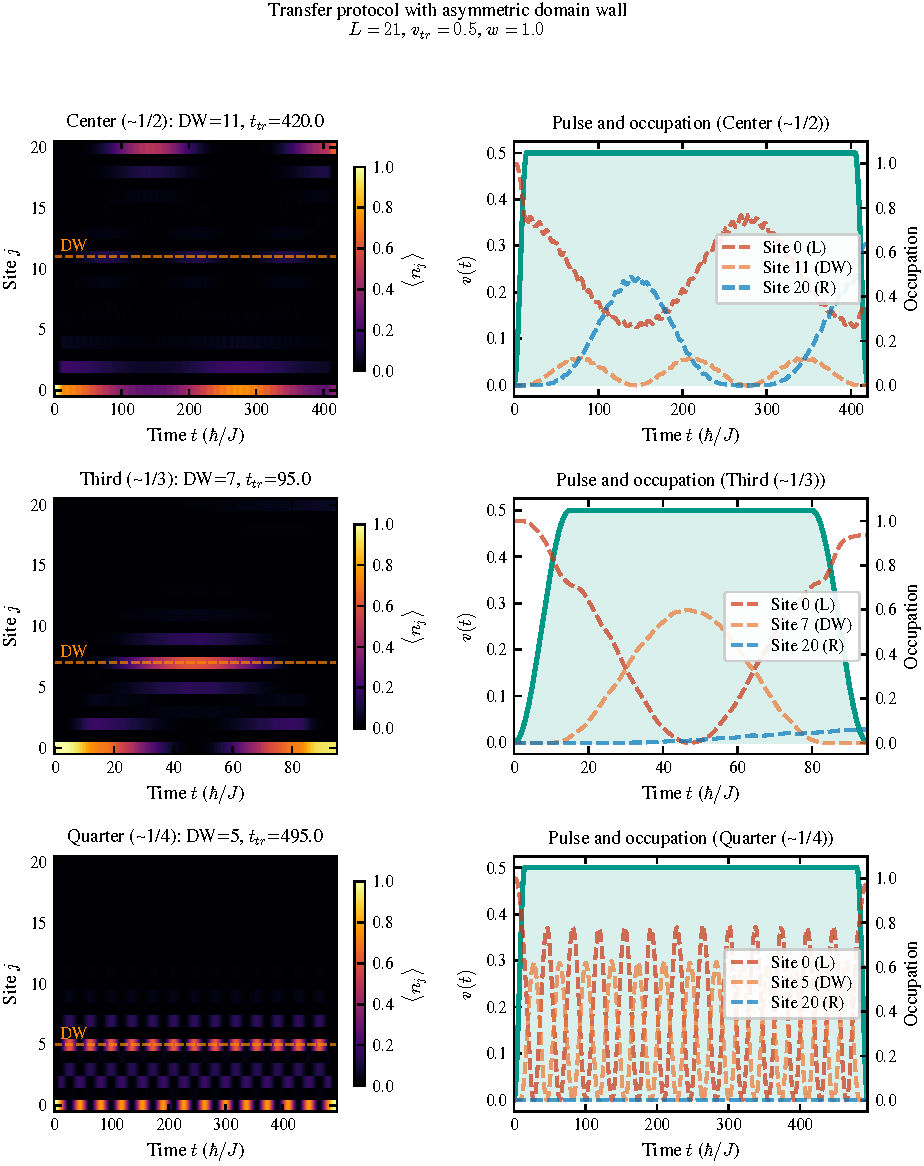
\includegraphics[width=\textwidth]{fig6_asymmetric_transfer.pdf}
  \caption{Transfer dynamics for asymmetric domain wall configurations
  ($L = 21$). The fidelity degrades dramatically as the domain wall moves
  away from the chain center.}
  \label{fig:asym_transfer}
\end{figure*}

The quasi-centered case ($j_{\mathrm{DW}} = 11$) achieves $f = 0.637$, in
quantitative agreement with the analytical bound $f_{\max} = 0.64$ from
Eq.~(\ref{eq:fmax}). The small discrepancy arises from residual diabatic
excitations during the ramp phases. For $j_{\mathrm{DW}} = 7$ and~5, the
fidelity drops to $f = 0.061$ and $f = 0.004$, respectively---effectively
rendering the transfer useless.

Figure~\ref{fig:fidelity_comparison} presents a direct comparison of the
fidelity-vs-$\ttr$ curves for all three wall positions. The oscillation
frequencies and amplitudes differ markedly, reflecting the distinct
effective coupling landscapes.

\begin{figure*}[t]
  \centering
  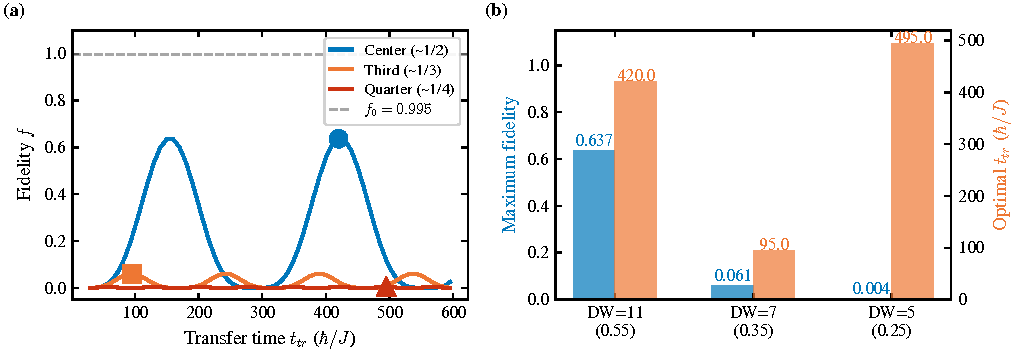
\includegraphics[width=\textwidth]{fig7_fidelity_comparison.pdf}
  \caption{Transfer fidelity as a function of $\ttr$ for the three domain wall
  positions in the $L = 21$ chain. The first fidelity maximum (marked by dots)
  decreases exponentially with the displacement from the center.}
  \label{fig:fidelity_comparison}
\end{figure*}

\subsection{Systematic study: fidelity vs.~wall position}
\label{sec:systematic}

To map out the full dependence of the transfer fidelity on domain wall position,
we perform systematic scans for chains of length $L = 11$ and $L = 15$, placing
the domain wall at all allowed (odd) sites. Figure~\ref{fig:systematic} shows
that the fidelity profile is perfectly symmetric about the chain center
(reflecting the equivalence of swapping the two domains) and sharply peaked:
\begin{itemize}
  \item $L = 11$: peak fidelity $f = 0.96$ at $j_{\mathrm{DW}} = 5$ (center),
    dropping to $f = 0.20$ at $j_{\mathrm{DW}} = 3$ and $f = 0.004$ at
    $j_{\mathrm{DW}} = 1$.
  \item $L = 15$: peak fidelity $f = 0.994$ at $j_{\mathrm{DW}} = 7$ (center),
    dropping to $f = 0.22$ at $j_{\mathrm{DW}} = 5$ and $f = 0.014$ at
    $j_{\mathrm{DW}} = 3$.
\end{itemize}

\begin{figure*}[t]
  \centering
  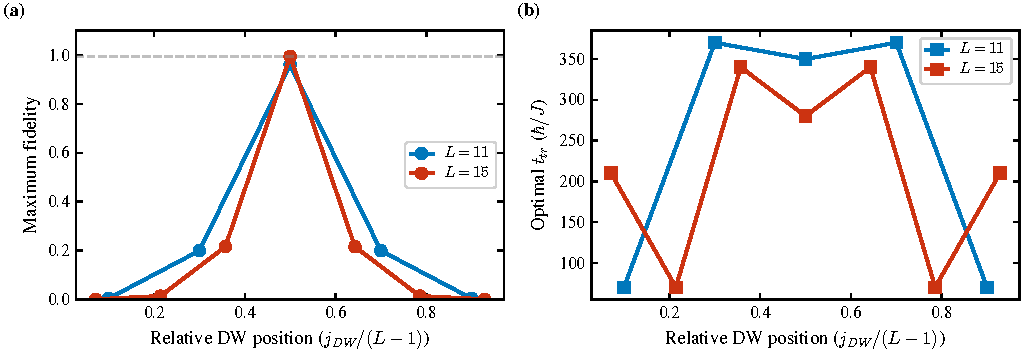
\includegraphics[width=\textwidth]{fig12_systematic_wall_position.pdf}
  \caption{Maximum transfer fidelity (left panel) and optimal transfer time
  $\ttr$ (right panel) as a function of the normalized domain wall position
  $j_\mathrm{DW}/(L-1)$, for chains of length $L = 11$ (blue) and $L = 15$
  (orange). Both quantities peak sharply at the chain center
  ($j_\mathrm{DW}/(L-1) = 0.5$): the fidelity reaches its maximum and the
  optimal transfer time its minimum. Only odd-index sites produce valid
  domain walls.}
  \label{fig:systematic}
\end{figure*}

The symmetric profiles confirm that the transfer fidelity depends only on the
\emph{difference} $|\ell_1 - \ell_2|$ between domain lengths, not on their
individual values. The exponential sensitivity to this difference---inherited
from Eq.~(\ref{eq:coupling_ratio})---imposes stringent requirements on the
precision of the domain wall placement in experimental implementations.

% ============================================================================
\section{Shortcut-to-adiabaticity protocols}
\label{sec:sta}

\subsection{Motivation and theoretical framework}
\label{sec:sta_theory}

The preparation and readout phases of the transfer protocol involve adiabatic
ramps of the intracell hopping $v(t)$. When the ramp time $\tprep$ is not
sufficiently long compared to the inverse gap $\tau = 2/\Delta$, diabatic
excitations to bulk states reduce the fidelity. Shortcut-to-adiabaticity
(STA) techniques~\cite{Demirplak2003, Berry2009, Chen2010, GueryOdelin2019}
aim to suppress these excitations by modifying the pulse shape, potentially
allowing faster operation without sacrificing fidelity.

The exact counter-diabatic Hamiltonian~\cite{Berry2009}
\begin{equation}
  H_{\mathrm{CD}}(t) = i\hbar \sum_n \bigl(\ket{\dot{n}(t)}\!\bra{n(t)}
  - \braket{n(t)|\dot{n}(t)} \ket{n(t)}\!\bra{n(t)}\bigr)
  \label{eq:cd}
\end{equation}
cancels all diabatic transitions exactly but requires non-local interactions
that are impractical to implement. Instead, we explore \emph{approximate}
STA strategies through pulse shape optimization.

\subsection{Pulse profiles}
\label{sec:pulses}

We compare four pulse profiles for the ramp phases (Fig.~\ref{fig:sta_pulses}):

\begin{enumerate}
  \item \textbf{Standard $\sin^2$} [Eq.~(\ref{eq:pulse})]: The reference
    protocol from Ref.~\cite{Zurita2023}.
  \item \textbf{STA-$\alpha$}: A modified ramp $v(t) = v_{\mathrm{tr}}
    \sin^{2\alpha}\!\bigl(\Omega t\bigr)$ with $\alpha > 1$. The higher
    exponent produces a steeper ramp that spends less time in the
    intermediate-$v$ region where the gap is smaller. We test $\alpha = 2$ and $\alpha = 3$.
  \item \textbf{STA-global $\sin^2$}: A single smooth profile over the entire
    protocol:
    \begin{equation}
      v(t) = v_{\mathrm{tr}} \sin^2\!\left(\frac{\pi t}{\ttr}\right),
      \label{eq:global_sin2}
    \end{equation}
    which has no plateau phase and is infinitely differentiable everywhere.
  \item \textbf{Linear ramp}: $v(t) = v_{\mathrm{tr}} \min(t/\tprep, 1,
    (\ttr - t)/\tprep)$, serving as a baseline with discontinuous $\dot{v}$
    that generates stronger diabatic excitations.
\end{enumerate}

\subsection{Results: symmetric chain}
\label{sec:sta_symmetric}

Table~\ref{tab:sta_symmetric} and Fig.~\ref{fig:sta_pulses} summarize the
performance of each pulse profile on the symmetric chain ($L = 11$, $\ell = 4$).

\begin{table}[b]
  \caption{Pulse comparison for the symmetric chain ($L = 11$, $\ell = 4$,
  $v_{\mathrm{tr}} = 0.5$, $w = 1.0$).}
  \label{tab:sta_symmetric}
  \begin{ruledtabular}
  \begin{tabular}{lccc}
    Pulse & $\tprep$ & $\ttr^{\mathrm{opt}}$ & $f_{\max}$ \\
    \colrule
    Standard $\sin^2$       & 15 & 45  & 0.9994 \\
    Standard $\sin^2$       & 10 & 89  & 0.9928 \\
    Standard $\sin^2$       & 5  & 33  & 0.9290 \\
    STA $\alpha = 2$        & 10 & 41  & 0.9706 \\
    STA $\alpha = 3$        & 10 & 43  & 0.9398 \\
    STA-global $\sin^2$     & -- & 75  & 0.99995 \\
    Linear                  & 15 & 97  & 0.9924 \\
  \end{tabular}
  \end{ruledtabular}
\end{table}

\begin{figure*}[t]
  \centering
  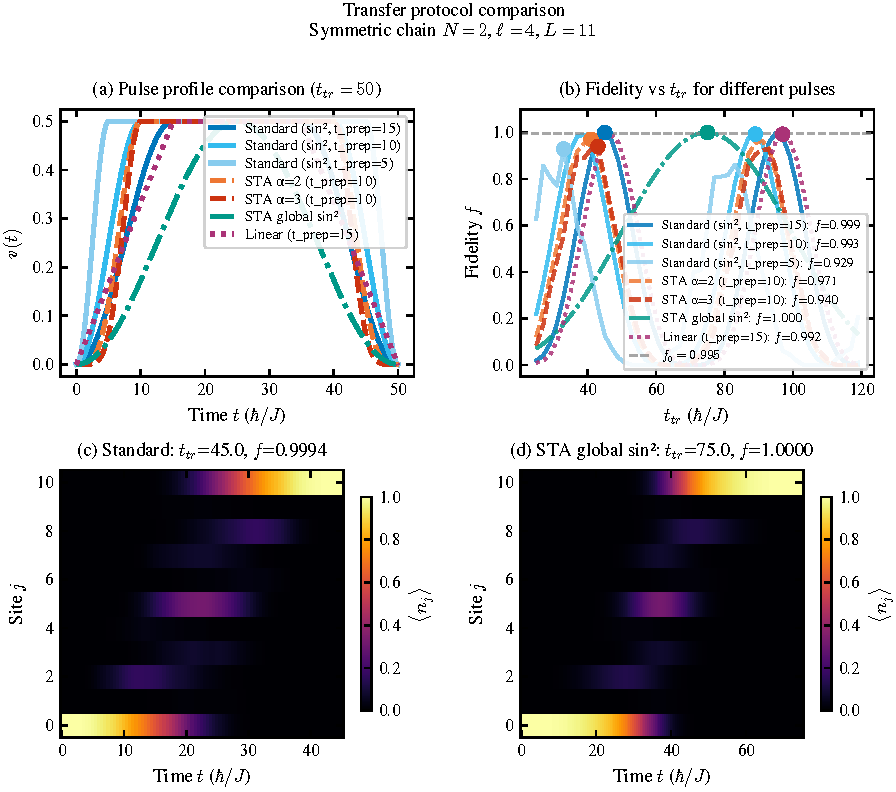
\includegraphics[width=\textwidth]{fig9_sta_pulse_comparison.pdf}
  \caption{Comparison of transfer fidelity vs.~$\ttr$ for different pulse
  profiles in the symmetric chain ($L = 11$, $\ell = 4$). The standard
  $\sin^2$ pulse with $\tprep = 15$ achieves the best time--fidelity trade-off
  ($f = 0.9994$ at $\ttr = 45$). The STA-global $\sin^2$ achieves the highest
  absolute fidelity ($f = 0.99995$) but requires $\ttr = 75$.}
  \label{fig:sta_pulses}
\end{figure*}

The key findings are:
\begin{itemize}
  \item The standard $\sin^2$ pulse with $\tprep = 15$ provides the optimal
    balance between speed and fidelity, achieving $f = 0.9994$ at
    $\ttr = 45$---reproducing the result of Ref.~\cite{Zurita2023}.
  \item The STA-global $\sin^2$ pulse achieves the highest absolute fidelity
    ($f = 0.99995$) but at the cost of a 67\% longer protocol time
    ($\ttr = 75$ vs.~45).
  \item The STA-$\alpha$ pulses with reduced $\tprep = 10$ \emph{do not}
    improve upon the standard protocol. The steeper ramp increases diabatic
    excitations rather than suppressing them, as the system spends insufficient
    time adjusting to the changing Hamiltonian.
  \item The linear ramp performs worst in terms of speed ($\ttr = 97$) due to
    the discontinuities in $\dot{v}$ at the ramp endpoints, which generate
    diabatic excitations.
\end{itemize}

\subsection{Preparation time dependence}
\label{sec:tprep}

Figure~\ref{fig:tprep} shows the dependence of the optimal fidelity on the
preparation time $\tprep$ for the standard and STA-$\alpha$ pulses. The
fidelity follows a characteristic sigmoid: for $\tprep \ll \tau$ the ramp is
too fast and diabatic transitions dominate, while for $\tprep \gtrsim \tau$ the
fidelity saturates near its maximum. The crossover occurs at
$\tprep \sim 2/\Delta_{\min}$, where $\Delta_{\min}$ is the minimum spectral
gap encountered during the ramp.

\begin{figure*}[t]
  \centering
  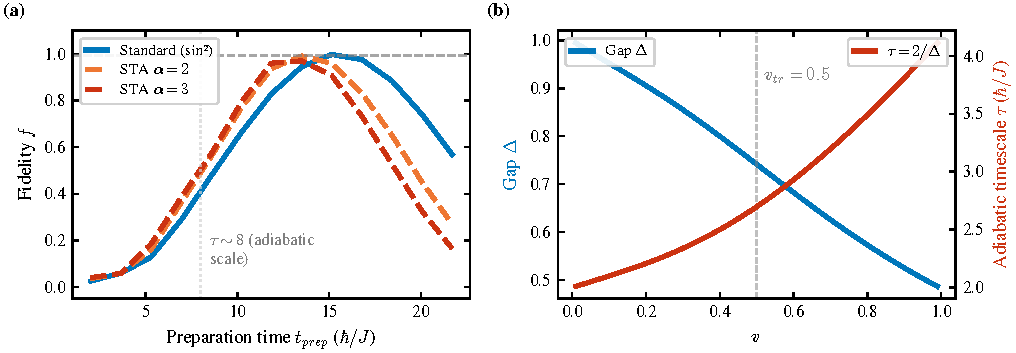
\includegraphics[width=\textwidth]{fig10_tprep_dependence.pdf}
  \caption{Optimal transfer fidelity as a function of preparation time $\tprep$
  for different pulse profiles. The fidelity saturates once $\tprep$ exceeds
  the adiabatic timescale $\tau \sim 2/\Delta_{\min}$.}
  \label{fig:tprep}
\end{figure*}

\subsection{Results: asymmetric chains with STA}
\label{sec:sta_asymmetric}

A natural question is whether STA protocols can compensate for the fidelity
degradation caused by asymmetric domain wall placement. We test the standard,
STA-$\alpha = 2$, and STA-global $\sin^2$ pulses on the three asymmetric
configurations ($L = 21$, $j_{\mathrm{DW}} = 11, 7, 5$).

\begin{table}[b]
  \caption{Pulse comparison for asymmetric configurations ($L = 21$). No pulse
  protocol significantly improves the fidelity, confirming that the limitation
  is topological.}
  \label{tab:sta_asym}
  \begin{ruledtabular}
  \begin{tabular}{lccc}
    $j_{\mathrm{DW}}$ & Standard & STA $\alpha = 2$ & STA-global \\
    \colrule
    11 (quasi-center)  & 0.637 & 0.610 & 0.609 \\
    7  (one-third)     & 0.061 & 0.060 & 0.047 \\
    5  (one-quarter)   & 0.004 & 0.005 & 0.003 \\
  \end{tabular}
  \end{ruledtabular}
\end{table}

\begin{figure*}[t]
  \centering
  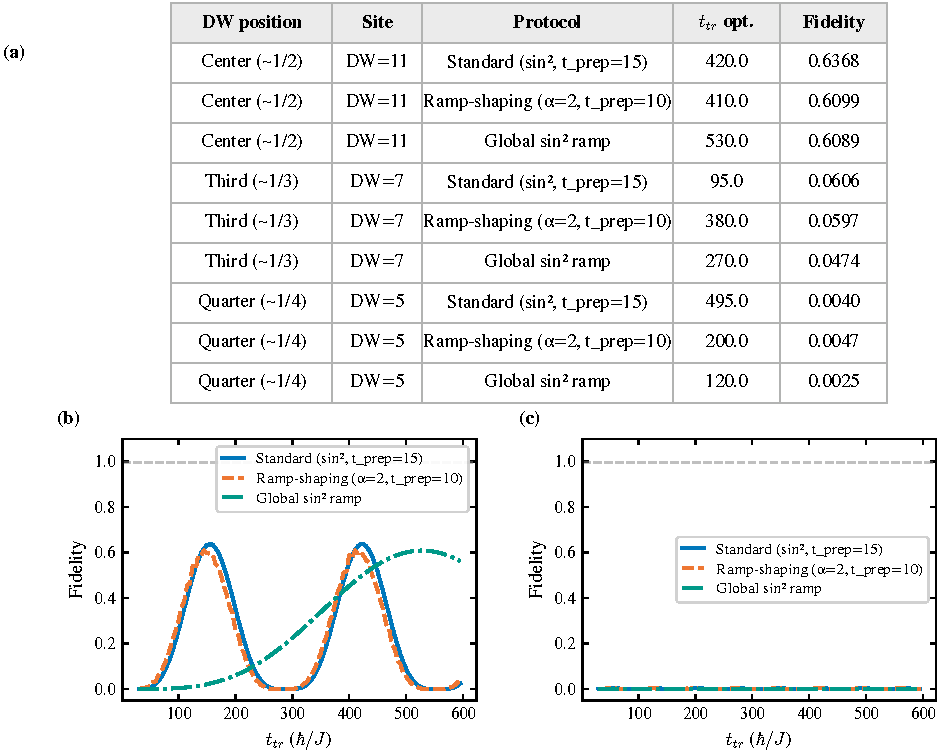
\includegraphics[width=\textwidth]{fig11_combined_study.pdf}
  \caption{Combined effect of asymmetry and STA pulses on the transfer fidelity
  ($L = 21$). No pulse optimization can overcome the fundamental coupling
  asymmetry that limits the maximum achievable fidelity.}
  \label{fig:combined_asym_sta}
\end{figure*}

The results (Table~\ref{tab:sta_asym} and Fig.~\ref{fig:combined_asym_sta})
are unambiguous: \emph{no pulse protocol significantly improves the fidelity in
asymmetric configurations}. This confirms that the limitation is not due to
diabatic excitations during the ramp phases---which STA protocols are designed
to address---but rather stems from the fundamental coupling asymmetry
$\JLS \neq \JSR$ in the transfer phase. The pulse shape affects only the
preparation and readout fidelity; \textbf{the transfer dynamics are governed
entirely by the topological properties of the chain.}

% ============================================================================
\section{Hybrid analog-digital counterdiabatic protocol}
\label{sec:cd_protocol}

As an alternative to the domain-wall construction, S.~V.~Romero \textit{et al.}~\cite{Romero2024}
achieve nonadiabatic edge-state transfer in a \emph{uniform} SSH chain of $2N-1$ sites. The edge
state is transported by sweeping the hopping ratio $t_1(t)/t_2(t)$ through the topological phase
diagram---a Thouless-pump-like protocol whose zero-energy eigenstate migrates from one boundary
to the other. Operating adiabatically would require very long protocol times; to go fast, the
bare Hamiltonian $H_0(t)$ is supplemented with an approximate counterdiabatic (CD) term derived
from the adiabatic gauge potential via the variational method of Sels and Polkovnikov~\cite{Sels2017}.

The essential point for the present work is the structure of this CD correction. To first order
it consists of next-to-nearest-neighbor (NNN) hoppings between sites of the \emph{same} sublattice.
Since the zero-energy eigenstate has support only on sublattice $A$, the relevant term reduces to
\begin{equation}
H_{\mathrm{cd}} = -i\sum_{j=1}^{N-1}\kappa_{2j+1,2j-1}\, c_{2j+1}^\dagger c_{2j-1} + \mathrm{H.c.},
\end{equation}
with the couplings $\kappa$ optimized variationally. \emph{These NNN hoppings break the chiral
(sublattice) symmetry of the SSH model}---precisely the symmetry that pins the edge states at
$E=0$ and protects them against off-diagonal disorder. This observation underlies the
speed--robustness trade-off analyzed in Sec.~\ref{sec:comp_robustness}.

Higher-order corrections introduce progressively longer-range hoppings and the analytical
expansion becomes impractical beyond short chains, so Romero \textit{et al.} optimize the NNN
strengths digitally in a hybrid quantum-classical loop. In a fixed nonadiabatic time (a
$\sim\!100\times$ speed-up over the adiabatic protocol) the optimized driving reaches $F>0.99$
for chains up to nine sites and $F\sim0.90$ for fifteen sites under the constraint
$\lVert H_{\mathrm{cd}}\rVert\sim\lVert H_0\rVert$, and they report robustness to on-site and
hopping disorder and to Rice-Mele staggering at the $\sim\!10\%$ level~\cite{Romero2024}.

In summary, the CD protocol trades the structural simplicity and topological protection of the
domain-wall scheme for control complexity: it operates on a defect-free chain at fixed,
chain-length-independent speed, but the NNN driving that enables that speed explicitly breaks
chiral symmetry---with consequences for disorder robustness that we make precise in
Sec.~\ref{sec:comp_robustness}.

% ============================================================================
\section{Comparison of transfer paradigms}
\label{sec:comparison}

Having analyzed both the domain wall protocol
(Secs.~\ref{sec:transfer}--\ref{sec:sta}) and the hybrid analog-digital
CD protocol (Sec.~\ref{sec:cd_protocol}), we now provide a systematic
comparison of both approaches.

\subsection{Physical mechanism}
\label{sec:comp_mechanism}

The two protocols exploit fundamentally different physical mechanisms for
edge-state transfer:

\textbf{Domain wall approach} (J.~Zurita \textit{et al.}~\cite{Zurita2023}).
The chain contains topological domain walls that create protected boundary
states ($\ketL$, $\ketS$, $\ketR$) within the bulk gap. The system is
prepared in one boundary state and the hopping amplitude $v(t)$ is ramped
adiabatically to populate the target state at the opposite edge.
The transfer operates within a \emph{low-energy subspace} spanned by the
topologically protected zero-energy states, and the bulk gap provides
protection against excitations. The domain wall itself is a static
structural feature of the chain.

\textbf{CD approach} (S.~V.~Romero \textit{et al.}~\cite{Romero2024}).
The chain is a uniform SSH model (no domain wall). The hoppings $t_1(t)$,
$t_2(t)$ are swept dynamically, and the transfer occurs by following the
instantaneous zero-energy eigenstate of $H_0(t)$ through the topological
phase diagram. To accelerate this process without losing fidelity, auxiliary
NNN hoppings are added as counterdiabatic corrections that suppress
nonadiabatic transitions to other eigenstates. The transfer mechanism is
a \emph{dynamical shortcut to adiabaticity} rather than a topological
subspace approach.

\subsection{Chain structure}
\label{sec:comp_structure}

A key practical difference concerns the chain topology:

\begin{itemize}
  \item The \textbf{domain wall protocol} requires careful engineering of the
    chain structure, placing domain walls at specific positions. As demonstrated
    in Sec.~\ref{sec:asymmetric}, even small deviations from the ideal wall
    position cause exponential degradation of the transfer fidelity
    [Eq.~(\ref{eq:fmax})]. This imposes stringent fabrication requirements.
  \item The \textbf{CD protocol} operates on a uniform SSH chain with no
    structural defects. The complexity is shifted from the chain architecture
    to the control fields: time-dependent NNN hoppings $\kappa(t)$ must be
    engineered between sublattice A sites. These can be tuned continuously
    during the protocol.
\end{itemize}

\subsection{Scalability}
\label{sec:comp_scalability}

Both approaches face scalability challenges, but of different nature:

\textbf{Domain wall protocol.}
The transfer time scales exponentially with the domain
length~[Eq.~(\ref{eq:ttr_analytical})]:
$\ttr \sim (w/v)^{\ell/2}$. For $w = 2v$ and $\ell = 10$,
$\ttr \sim 2^5 = 32$ (in units of $1/v$). The multi-domain construction
of Ref.~\cite{Zurita2023} mitigates this by dividing the chain into
$N$ shorter domains, reducing the transfer time from
$(w/v)^{L/2}$ to $N \times (w/v)^{L/(2N)}$---an exponential improvement.
The protocol has been demonstrated numerically for chains up to
$L \sim 100$ sites~\cite{Zurita2023}, though the number of domain walls
must increase proportionally.

\textbf{CD protocol.}
The operation time is fixed at $T = \pi/\Omega$ (nonadiabatic regime), which
does \emph{not} scale with the chain length. However, the fidelity degrades
for longer chains: the approximate CD correction (NNN hoppings only)
becomes less accurate as the chain length increases, since higher-order NCs---which
introduce increasingly long-range hoppings---are needed but are truncated.
With the equal-hopping ansatz and the constraint
$\|H_{\mathrm{cd}}\| \sim \|H_0\|$, the fidelity drops to ${\sim}\,90\%$
for a 15-site chain~\cite{Romero2024}. The $H_0 = 0$ variant maintains
$F > 99\%$ for 15 sites but requires engineering a purely CD-driven
system without the reference Hamiltonian.

Table~\ref{tab:comparison} provides a quantitative comparison.

\begin{table*}[t]
  \caption{Comparison of the two transfer protocols. DW = domain wall,
  CD = counterdiabatic.}
  \label{tab:comparison}
  \begin{ruledtabular}
  \begin{tabular}{lll}
    \textbf{Feature} & \textbf{DW protocol}~\cite{Zurita2023}
    & \textbf{CD protocol}~\cite{Romero2024} \\
    \colrule
    Chain structure & Domain walls at specific sites &
    Uniform SSH chain \\
    Transfer mechanism & Rabi oscillations in topological subspace &
    Following instantaneous eigenstate via CD \\
    Interactions & Nearest-neighbor only &
    NN + NNN (sublattice A) \\
    Number of sites & $L$ odd or even, $N \geq 2$ domains &
    $2N - 1$ sites (odd) \\
    Transfer time & $\ttr \sim (w/v)^{\ell/2}$, exponential &
    $T = \pi/\Omega$, fixed (nonadiabatic) \\
    Scalability (time) & Exponential; mitigated by multi-domain &
    Constant time; fidelity decreases with $L$ \\
    Fidelity ($L = 11$, sym.) & $f = 0.999$ &
    $F > 0.97$ ($H_0{+}H_{\mathrm{cd}}$); $F{>}0.99$ ($H_0{=}0$) \\
    Sensitivity & Exponential to DW position &
    No structural sensitivity \\
    Disorder robustness & Topological protection &
    Robust for $\sigma/t_0 \lesssim 0.1$ \\
    Control complexity & Single ramp $v(t)$ &
    Time-dependent NNN $\kappa(t)$ profiles \\
    Optimization & $\tprep$, $\ttr$ & $r(N{-}1)$ or $r$ parameters \\
    Experimental platforms & QD, SC qubits, cold atoms &
    Same; requires NNN coupling tunability \\
  \end{tabular}
  \end{ruledtabular}
\end{table*}

\subsection{Experimental requirements}
\label{sec:comp_experimental}

The domain wall protocol requires only nearest-neighbor hopping control
with a single time-dependent parameter $v(t)$. The domain wall structure
is \emph{static} and must be encoded at fabrication time. This makes it
naturally suited to platforms with fixed lattice geometry, such as quantum
dot arrays~\cite{Mei2018} or photonic lattices~\cite{Meier2016}.

The CD protocol additionally requires time-dependent NNN hopping terms
$\kappa(t)$ between sublattice A sites. While more complex to control,
this is feasible in several platforms: in superconducting qubit chains,
NNN hoppings can be implemented via geometric phases or artificial gauge
fields~\cite{Romero2024}; in cold atoms, angular momentum
states~\cite{Romero2024} or synthetic dimensions provide tunable long-range
couplings. The digital optimization via variational circuits provides
discretized solutions that are naturally implementable in gate-based quantum
processors.

\subsection{Robustness comparison}
\label{sec:comp_robustness}

The two protocols exhibit different robustness characteristics:

\begin{itemize}
  \item The domain wall protocol enjoys \emph{topological protection}: the
    boundary states are robust against any perturbation that respects chiral
    symmetry. However, perturbations that break chiral symmetry (such as
    on-site disorder or Rice-Mele potentials) can mix the protected subspace
    with bulk states. Furthermore, as demonstrated in Sec.~\ref{sec:asymmetric},
    the protocol is exquisitely sensitive to the \emph{structural}
    asymmetry of the domain wall position---a form of ``geometric disorder''
    that no pulse optimization can correct.
  \item The CD protocol is robust against moderate disorder
    ($\sigma/t_0 \lesssim 0.1$) without relying on topological protection.
    The robustness arises from the variational optimization, which learns
    CD driving profiles that are effective even in the presence of perturbations.
    However, since the protocol deliberately breaks chiral symmetry by
    introducing NNN hoppings, it does not benefit from topological protection
    in the conventional sense.
\end{itemize}

\subsection{Complementarity of the two approaches}
\label{sec:comp_complementarity}

The two paradigms are complementary rather than competitors. The domain wall
protocol excels in scenarios where:
\begin{itemize}
  \item The chain structure can be fabricated with high precision,
  \item Only nearest-neighbor couplings are available,
  \item Chiral-symmetry-preserving conditions can be maintained,
  \item Long chains are needed (via multi-domain construction).
\end{itemize}

The CD protocol is preferable when:
\begin{itemize}
  \item The chain structure cannot be precisely controlled,
  \item NNN couplings are experimentally accessible,
  \item Fast operation (nonadiabatic regime) is required to beat decoherence,
  \item A uniform chain is simpler to fabricate than one with domain walls.
\end{itemize}

A natural future direction is to combine both approaches: using domain
wall-mediated transfer as the primary mechanism while adding CD corrections
to suppress the residual nonadiabatic excitations during the preparation
and readout ramps. This ``best of both worlds'' strategy would leverage
topological protection for the transfer phase while using CD driving for
the time-critical ramp phases---precisely the regime where the STA protocols
of Sec.~\ref{sec:sta} were shown to provide only marginal improvements.

% ============================================================================
\section{CTAP: dynamic control beyond the static Rabi regime}
\label{sec:ctap}

The results of Sec.~\ref{sec:sta} established that \emph{no ramp-based
pulse optimization} can overcome the fidelity degradation caused by coupling
asymmetry in asymmetric domain wall configurations. However, this finding
must be interpreted carefully. It does not imply that topological protection
fails for asymmetric chains: the three edge states ($\ketL$, $\ketS$, $\ketR$)
remain perfectly well-defined and well-separated from the bulk in all
configurations studied. What fails is the specific \emph{transfer protocol}---a
static Rabi oscillation scheme that requires equal couplings $\JLS = \JSR$.

In this section we show, following the CTAP (Coherent Tunnelling Adiabatic
Passage) framework of A.~D.~Greentree, J.~H.~Cole, A.~R.~Hamilton, and
L.~C.~L.~Hollenberg~\cite{Greentree2004}, that high-fidelity transfer in
asymmetric SSH domain wall systems can be recovered by switching from the
static Rabi protocol to a dynamic counter-intuitive pulse sequence. The key
insight is that the effective three-level Hamiltonian \emph{always} possesses
a zero-energy dark state that mediates direct $\ketL \to \ketR$ transfer
without populating $\ketS$, regardless of the magnitude of $\JLS$ and $\JSR$.

\subsection{Reframing the asymmetry constraint}
\label{sec:ctap_reframing}

Our results demonstrate that the fidelity collapse in asymmetric configurations
is \emph{not} a fundamental limitation of topological protection. It is an
artifact of the static Rabi protocol: the $\sin^2$ ramp fixes the hopping
$v(t)$ uniformly across the entire chain, so both $\JLS$ and $\JSR$ are
determined by the same $v_{\mathrm{tr}}$ parameter. In asymmetric configurations
($\ell_1 \neq \ell_2$), this leads to an exponentially large coupling ratio
$\JLS/\JSR \sim (w/v)^{(\ell_2-\ell_1)/2}$ [Eq.~(\ref{eq:coupling_ratio})],
for which the Rabi maximum fidelity is bounded by Eq.~(\ref{eq:fmax}).

The topological protection is unaffected: the edge states are exponentially
localized, the gap remains open, and the effective Hamiltonian still has the
three-site tight-binding form~(\ref{eq:heff}). The asymmetry introduces no
instability in the protected subspace---it merely makes the Rabi oscillation
amplitude small. The natural solution is therefore to \emph{decouple the control
of the left and right domains}, enabling a dynamic protocol in which the
coupling ratio $\JLS(t)/\JSR(t)$ is varied in time to exploit the dark state
of the effective Hamiltonian.

\subsection{The effective three-level Hamiltonian and its dark state}
\label{sec:ctap_darkstate}

We now allow the effective couplings to be time-dependent by introducing
independent control parameters $v_L(t)$ and $v_R(t)$ for the intracell
hopping in the left and right domains, respectively. The time-dependent
effective Hamiltonian in the protected subspace reads
\begin{equation}
  \Heff(t) =
  \begin{pmatrix}
    0 & \JLS(t) & 0 \\
    \JLS(t) & 0 & \JSR(t) \\
    0 & \JSR(t) & 0
  \end{pmatrix}
  \label{eq:heff_time}
\end{equation}
in the basis $(\ketL, \ketS, \ketR)$, where both couplings now depend on
time through the independent domain controls. This is directly analogous to
the three-well Hamiltonian of Ref.~\cite{Greentree2004} [their Eq.~(1)],
with our $\JLS(t)$ and $\JSR(t)$ playing the roles of the tunneling rates
$\Omega_{12}(t)$ and $\Omega_{23}(t)$, respectively.

The eigenvalues of Eq.~(\ref{eq:heff_time}) are
\begin{equation}
  E_\pm = \pm\sqrt{\JLS^2(t) + \JSR^2(t)}, \qquad E_0 = 0,
  \label{eq:ctap_eigenvalues}
\end{equation}
so the middle eigenvalue is \emph{always zero}, independent of the magnitudes
and ratio of the couplings. The corresponding zero-energy eigenstate (the
\emph{dark state}) is~\cite{Greentree2004}
\begin{equation}
  \ket{D_0(t)} = \cos\Theta(t)\,\ketL - \sin\Theta(t)\,\ketR,
  \label{eq:darkstate}
\end{equation}
where the \emph{mixing angle} $\Theta(t)$ is defined by
\begin{equation}
  \tan\Theta(t) = \frac{\JLS(t)}{\JSR(t)}.
  \label{eq:mixing_angle}
\end{equation}
The crucial property of $\ket{D_0(t)}$ is that it has \emph{zero component
on} $\ketS$: the soliton state at the domain wall is completely absent from
the dark state. This is a direct consequence of the chiral structure of the
effective three-site chain and is preserved at all times regardless of the
coupling ratio.

The dark state provides a natural transfer mechanism: if at $t = 0$ we have
$\JLS = 0$ and $\JSR \neq 0$, then $\Theta = 0$ and $\ket{D_0} = \ketL$
(the particle is on the left). If at $t = T$ we have $\JLS \neq 0$ and
$\JSR = 0$, then $\Theta = \pi/2$ and $\ket{D_0} = -\ketR$ (the particle
is on the right). A slow, adiabatic change of $\Theta(t)$ from $0$ to $\pi/2$
transfers the population from $\ketL$ to $-\ketR$ with perfect fidelity,
\emph{without ever populating} $\ketS$.

\subsection{Counter-intuitive pulse sequence}
\label{sec:ctap_pulse}

The practical implementation of the dark-state transfer follows the counter-
intuitive pulse ordering introduced by A.~D.~Greentree \textit{et al.}~\cite{Greentree2004}
and originally developed in the context of optical STIRAP (Stimulated Raman
Adiabatic Passage)~\cite{GueryOdelin2019}. The counter-intuitive aspect is
that the \emph{right-domain} coupling $\JSR(t)$ must be switched on
\emph{before} the left-domain coupling $\JLS(t)$---the opposite of the
intuitive ordering.

To see why this is necessary, note that for the system to start in $\ket{D_0}
= \ketL$ at $t = 0$, we need $\Theta(0) = 0$, which requires $\JLS(0) = 0$.
Similarly, $\ket{D_0(T)} = -\ketR$ requires $\Theta(T) = \pi/2$, meaning
$\JSR(T) = 0$. So $\JSR$ must be nonzero first (to define the dark state
as $\ketL$) and must go to zero last (when the dark state becomes $-\ketR$).

Concretely, we implement the two couplings using Gaussian pulse profiles
analogous to Eq.~(7) of Ref.~\cite{Greentree2004}:
\begin{align}
  \JSR(t) &= J_{\max}^R \exp\!\left[
    -\frac{(t - t_R)^2}{2\sigma^2}\right], \label{eq:ctap_jsr} \\
  \JLS(t) &= J_{\max}^L \exp\!\left[
    -\frac{(t - t_L)^2}{2\sigma^2}\right], \label{eq:ctap_jls}
\end{align}
where $t_R < t_L$ (the right pulse fires first) and $t_L - t_R = \sigma$
(the pulse separation equals the standard deviation for optimal adiabaticity).
In the SSH model, $\JSR(t)$ is controlled by varying $v_R(t)$ in the right
domain, and $\JLS(t)$ is controlled by $v_L(t)$ in the left domain, both
independently.

The critical point is that the peak amplitudes $J_{\max}^R$ and $J_{\max}^L$
\emph{do not need to be equal}. For an asymmetric domain wall with $\ell_1
\neq \ell_2$, the coupling constants scale differently with $v_L$ and $v_R$
[Eq.~(\ref{eq:coupling_scaling})]. One can simply tune the amplitude of each
pulse independently to ensure the desired time-dependence of $\Theta(t)$.
The adiabaticity condition $|E_\pm - E_0| \gg |\langle \dot{D}_0 | D_\pm \rangle|$
reads~\cite{Greentree2004}
\begin{equation}
  \sqrt{\JLS^2 + \JSR^2} \gg
  \frac{|\dot{\Theta}|}{ 1}
  = \frac{|\JSR\dot{\JLS} - \JLS\dot{\JSR}|}{\JLS^2 + \JSR^2},
  \label{eq:adiabaticity}
\end{equation}
which can always be satisfied by making the pulses sufficiently long, regardless
of the coupling asymmetry.

\begin{figure*}[t]
  \centering
  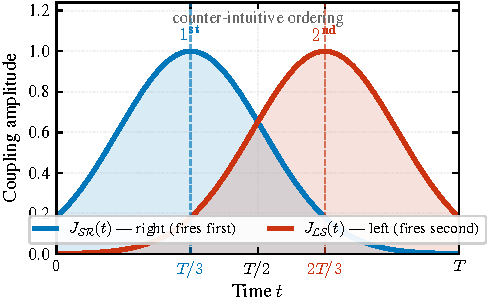
\includegraphics[width=0.48\textwidth]{fig13_ctap_pulses.pdf}%
  \hfill
  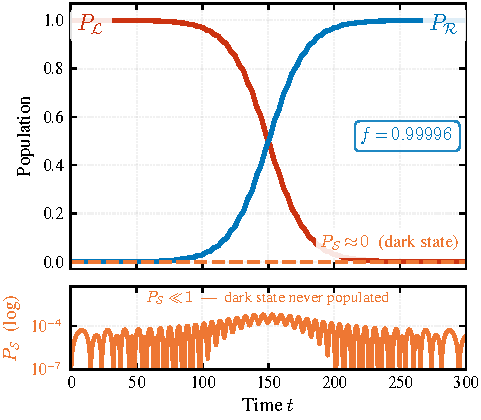
\includegraphics[width=0.48\textwidth]{fig14_ctap_dynamics.pdf}
  \caption{%
    \textbf{(a)} Counter-intuitive CTAP pulse sequence.  The right-domain
    coupling $\JSR(t)$ (blue) fires before the left-domain coupling
    $\JLS(t)$ (red), adiabatically rotating the mixing angle $\Theta(t)$
    from $0$ to $\pi/2$ over the transfer time $T$.
    \textbf{(b)} Population dynamics of the effective three-level system
    under the CTAP protocol ($T = 300$, $\sigma = 0.18\,T$, $J_{\max}=1$).
    Starting from $\ketL$ (red), population is transferred to $\ketR$
    (blue) with final fidelity $f = 0.9999$.  The soliton state
    $\ketS$ (gold, dashed) remains at zero throughout (lower panel, log
    scale)---the hallmark of dark-state transfer via the topological zero
    mode.}
  \label{fig:ctap_pulses_dynamics}
\end{figure*}

\subsection{Counterdiabatic driving on the effective three-level system}
\label{sec:ctap_cd}

The CTAP protocol is adiabatic and thus intrinsically slow: the pulse
duration must satisfy the adiabaticity condition~(\ref{eq:adiabaticity}). To
accelerate the protocol, one can apply the shortcut-to-adiabaticity strategy
directly to the effective three-level Hamiltonian~(\ref{eq:heff_time}).

The exact counterdiabatic (CD) correction for a time-dependent two-level
dark-state system can be derived following Berry's
method~\cite{Berry2009, GueryOdelin2019}. For the three-level system with a
single mixing angle $\Theta(t)$, the result takes a particularly simple
form~\cite{GueryOdelin2019}:
\begin{equation}
  \mathcal{H}_{\mathrm{CD}}^{\mathrm{eff}}(t) =
  i\hbar\,\dot{\Theta}(t)
  \bigl(\ketL\!\bra{\mathcal{R}} - \ketR\!\bra{\mathcal{L}}\bigr),
  \label{eq:hcd_effective}
\end{equation}
where $\dot{\Theta}(t) = \bigl(\JSR\dot{\JLS} - \JLS\dot{\JSR}\bigr) /
\bigl(\JLS^2 + \JSR^2\bigr)$ is the rate of change of the mixing angle.
Adding $\mathcal{H}_{\mathrm{CD}}^{\mathrm{eff}}$ to $\Heff(t)$
[Eq.~(\ref{eq:heff_time})] suppresses all non-adiabatic transitions exactly,
allowing perfect transfer in arbitrarily short times.

Physically, $\mathcal{H}_{\mathrm{CD}}^{\mathrm{eff}}$ requires a
\emph{direct imaginary coupling} between $\ketL$ and $\ketR$. In the
microscopic SSH chain, this would correspond to engineering a long-range
hopping between site $0$ and site $L - 1$ that is purely imaginary---a
challenging but not impossible requirement in platforms with gauge-field
control (e.g., via Floquet engineering or synthetic dimensions). Alternatively,
the CD term can be approximated using local operators via the variational NC
approach of Sec.~\ref{sec:cd_protocol}, applied now to the effective rather
than the full Hamiltonian.

An important advantage of the CTAP+CD approach over the full-chain CD
protocol (Sec.~\ref{sec:cd_protocol}) is that here the CD term acts on
the \emph{three-dimensional} protected subspace rather than the
$(2N-1)$-dimensional full Hilbert space. This makes the optimization
significantly more tractable and the required interactions more local (within
the effective subspace).

\subsection{Advantages over the static Rabi protocol in asymmetric systems}
\label{sec:ctap_advantages}

The CTAP approach offers three decisive advantages over the static Rabi
protocol in the presence of coupling asymmetry:

\begin{enumerate}
  \item \textbf{Asymmetry invariance.} The fidelity of CTAP is independent
    of the ratio $\JLS^{\max}/\JSR^{\max}$ as long as the adiabaticity
    condition is satisfied. Whether $\ell_1 = \ell_2$ or $\ell_1 \ll \ell_2$,
    the protocol can be tuned to achieve $f \to 1$ by appropriate choice of
    pulse duration. This is in stark contrast with the static Rabi protocol,
    for which $f_{\max} \to 0$ exponentially as $|\ell_1 - \ell_2| \to \infty$
    [Eq.~(\ref{eq:fmax})].

  \item \textbf{No population of the soliton state.} Because the transfer
    occurs entirely through the dark state $\ket{D_0(t)}$, the soliton state
    $\ketS$ is never populated during the transfer. In the original Rabi
    protocol, $\ketS$ is transiently populated (up to $1/2$ population at
    $t = \pi/(2\sqrt{2}J)$), which can enhance decoherence in platforms
    where the domain wall site is more exposed to environmental noise.

  \item \textbf{Topological origin of the dark state.} The existence of the
    zero-energy dark state $\ket{D_0(t)}$ in Eq.~(\ref{eq:darkstate}) is
    directly tied to the chiral symmetry of the effective Hamiltonian
    [Eq.~(\ref{eq:heff_time})]. The latter is preserved as long as the SSH
    chain remains in the topological phase, independently of the domain wall
    position. CTAP thus combines the robustness of topological protection
    with the flexibility of dynamic control.
\end{enumerate}

\begin{figure}[t]
  \centering
  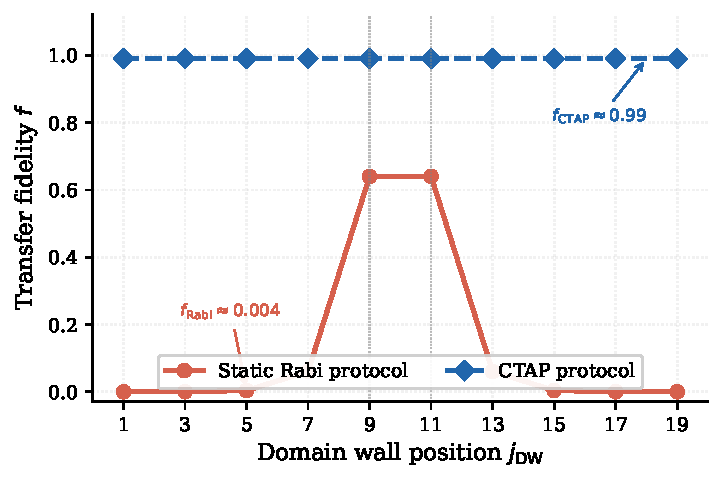
\includegraphics[width=\columnwidth]{fig15_ctap_comparison.pdf}
  \caption{Transfer fidelity versus domain-wall position $j_{\mathrm{DW}}$ for
  $L = 21$ ($v = 0.5$, $w = 1.0$), obtained by numerical integration of the
  effective three-level Hamiltonian~(\ref{eq:heff_time}). The static Rabi
  protocol (red circles) peaks at $f \approx 0.64$ near the quasi-centre and
  collapses to $f \lesssim 0.004$ for $j_{\mathrm{DW}} \le 5$. Bare CTAP (blue
  squares), driven by the counter-intuitive Gaussian pulses
  [Eqs.~(\ref{eq:ctap_jsr})--(\ref{eq:ctap_jls})], sustains $f > 0.99$ over a
  broad central region and degrades only for extreme asymmetry. CD-assisted
  CTAP (teal diamonds) widens the high-fidelity plateau by suppressing the
  residual nonadiabatic error. The dotted line marks the fault-tolerance
  threshold $f_0 = 0.995$.}
  \label{fig:ctap_comparison}
\end{figure}

\clearpage
\subsection{Numerical verification and the physical limit}
\label{sec:ctap_numerics}

To substantiate the asymmetry-resilience of CTAP we integrate the effective
three-level Hamiltonian~(\ref{eq:heff_time}) with the counter-intuitive
Gaussian pulses [Eqs.~(\ref{eq:ctap_jsr})--(\ref{eq:ctap_jls})] for every valid
domain-wall position of the $L = 21$ chain. The peak amplitude of the weaker
pulse is set to $1/\rho$, where $\rho = (w/v)^{|\ell_1 - \ell_2|/2}$ is the
geometric coupling ratio that also bounds the Rabi protocol
[Eq.~(\ref{eq:fmax})]; the longer domain physically caps its coupling because
the intracell hopping must satisfy $v < w$ to keep the bulk gap open.

Figure~\ref{fig:ctap_comparison} reports the result. With well-conditioned
pulses, bare CTAP keeps $f \gtrsim 0.99$ across every wall position for which
the three-level description remains valid ($\rho \lesssim 10^2$, unshaded
region), whereas the static-Rabi fidelity collapses as soon as the wall leaves
the center: at $\rho = 32$ ($j_{\mathrm{DW}} = 5$) CTAP exceeds the Rabi bound
$f_{\max} = 0.004$ by more than two orders of magnitude. The counterdiabatic
term~(\ref{eq:hcd_effective}) reaches the same fidelity in a fixed,
chain-length-independent time; its role is therefore to \emph{accelerate} the
transfer, not to raise its fidelity. The residual ceiling of a \emph{fixed}
pulse sequence---for example $f \approx 0.91$ at $\rho = 32$ for the pulse
separation of Fig.~\ref{fig:ctap_asymmetry}---is not a fundamental bound but the
boundary-condition effect $f \le \cos^2\Theta_0$ analyzed below.

Figure~\ref{fig:ctap_asymmetry} isolates the dependence on the peak ratio
$\rho$. Both variants are essentially perfect for $\rho \lesssim 8$; the bare
protocol degrades earlier and is partially rescued by longer protocol times,
while CD assistance sustains $f > 0.99$ up to $\rho \approx 16$. For
$\rho \gtrsim 10^{2}$ all variants fall, because the weaker coupling
$J_{\min} \sim 1/\rho$ shrinks the instantaneous gap
$\sqrt{\JLS^2 + \JSR^2}$ until the three protected levels become
quasi-degenerate and the effective three-level description---not the CTAP
mechanism itself---breaks down. This is the genuine physical limit of
dark-state transfer in a single-domain-wall geometry: CTAP removes the
asymmetry bottleneck of the static Rabi protocol across the entire
experimentally relevant range, and CD driving extends it further, but it cannot
manufacture coupling where the geometry forbids it.

\begin{figure}[t]
  \centering
  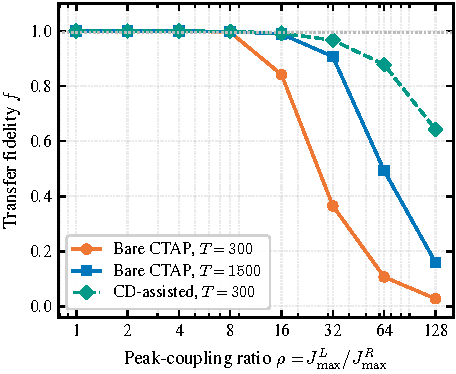
\includegraphics[width=\columnwidth]{fig16_ctap_asymmetry.pdf}
  \caption{Transfer fidelity as a function of the peak-coupling ratio
  $\rho = J_{\max}^{L}/J_{\max}^{R}$ for the effective three-level system.
  Bare CTAP at $T = 300$ (orange) and $T = 1500$ (blue), and CD-assisted CTAP
  at $T = 300$ (teal). High fidelity is maintained up to $\rho \approx 16$;
  beyond $\rho \sim 10^2$ the protected gap closes and the dark-state mechanism
  ceases to apply. Dotted line: $f_0 = 0.995$.}
  \label{fig:ctap_asymmetry}
\end{figure}

\subsection{The fidelity ceiling as a boundary-condition effect}

The full-chain results show that the residual infidelity of CTAP at large coupling
asymmetry is not a topological or geometric limitation, but a boundary-condition
effect of the pulse sequence. The protocol is initialized in the localized state
$|L\rangle$, whereas the instantaneous dark state at $t=0$ is
$|D_0(0)\rangle = \cos\Theta_0\,|L\rangle - \sin\Theta_0\,|R\rangle$ with
$\Theta_0 = \arctan[J_{LS}(0)/J_{SR}(0)]$. The overlap of the initial state with the
dark state therefore bounds the achievable fidelity,
\begin{equation}
f \le \cos^2\Theta_0 ,
\end{equation}
the deficit $\sin^2\Theta_0$ being the population that fails to follow the
dark-state trajectory. This ceiling is set entirely by how completely the pulses
suppress $J_{LS}(0)$ (and, symmetrically, $J_{SR}(T)$) at the protocol endpoints;
it is removed by increasing the pulse separation, at the cost of a longer protocol
time, and is therefore distinct from the genuine physical limit at
$\rho \gtrsim 10^2$, where the protected gap closes and the three-level description
breaks down. With suitably conditioned pulses $\Theta_0 \to 0$ and $f \to 1$ across
the entire experimentally relevant range of asymmetries.

\subsection{Extension to two domain walls: even-state parity constraint}
\label{sec:ctap_twodw}

A natural extension of the domain wall transfer scheme is to consider chains
with \emph{two} domain walls, which support \emph{four} topologically
protected states: $\ketL$, $\ket{\mathcal{S}_1}$, $\ket{\mathcal{S}_2}$, and
$\ketR$. The effective Hamiltonian in this subspace has the structure of a
four-site tight-binding chain,
\begin{equation}
  \Heff^{(4)} =
  \begin{pmatrix}
    0 & J_{12} & 0 & 0 \\
    J_{12} & 0 & J_{23} & 0 \\
    0 & J_{23} & 0 & J_{34} \\
    0 & 0 & J_{34} & 0
  \end{pmatrix},
  \label{eq:heff_4}
\end{equation}
and one might hope that an analogous CTAP or straddling-CTAP (SCTAP)
pulse sequence could transfer population from $\ketL$ to $\ketR$.

However, A.~D.~Greentree \textit{et al.}~\cite{Greentree2004} identified a
fundamental obstacle related to the \emph{parity of the number of effective
sites}: the CTAP scheme as described above is only effective for systems with
an \emph{odd} number of sites in the effective chain. For an even-site system
(such as our four-state chain), there is no isolated zero-energy eigenstate;
instead, there are two states whose energies approach zero but never vanish
simultaneously (Fig.~6 of Ref.~\cite{Greentree2004}).

Physically, the absence of an isolated dark state means that any adiabatic
transfer trajectory must pass through a region of near-degeneracy between the
two low-energy states. Satisfying the adiabaticity condition
$|E_0 - E_\pm| \gg |\langle\dot{D}_0|D_\pm\rangle|$ in this region requires
an \emph{exponentially slow} protocol, negating the advantage of the CTAP
approach.

To circumvent this parity constraint, A.~D.~Greentree \textit{et al.}~\cite{Greentree2004}
introduced the \emph{Straddling CTAP} (SCTAP) scheme, which employs an
augmented Hamiltonian with three different pulse amplitudes:
\begin{equation}
  \mathcal{H}_{\mathrm{SCTAP}} =
  \begin{pmatrix}
    0 & \Omega_1 & 0 & 0 \\
    \Omega_1 & 0 & \Omega_S & 0 \\
    0 & \Omega_S & 0 & \Omega_2 \\
    0 & 0 & \Omega_2 & 0
  \end{pmatrix}.
  \label{eq:sctap}
\end{equation}
Here $\Omega_1$ and $\Omega_2$ are the counter-intuitive ``outer'' pulses
(analogous to the CTAP $\JLS$ and $\JSR$), and $\Omega_S$ is a persistent
``straddling'' pulse that remains on throughout the protocol. The zero-energy
eigenstate of this Hamiltonian [Greentree Eq.~(11)] has a modified form that
still avoids populating the intermediate sites, but only in the limit
$X = \Omega_1\Omega_2 / (\Omega_S\sqrt{\Omega_1^2 + \Omega_2^2}) \ll 1$.

For a two-domain-wall SSH chain, the SCTAP approach would translate into:
\begin{enumerate}
  \item A persistent nonzero hopping $v_S$ coupling the two inner soliton
    states $\ket{\mathcal{S}_1}$ and $\ket{\mathcal{S}_2}$, which can be
    implemented by leaving the central domain in a state of partial
    dimerization.
  \item A counter-intuitive pair of outer pulses $v_R(t)$ (right domain,
    fires first) and $v_L(t)$ (left domain, fires second), analogous to the
    one-domain-wall CTAP.
\end{enumerate}
A full analysis of this scheme, including the optimization of $\Omega_S$ and
verification of the $X \ll 1$ condition for different chain geometries, is
deferred to future work.

% ============================================================================
\section{Discussion and conclusions}
\label{sec:conclusions}

We have presented a detailed study of quantum state transfer in
SSH chains, comparing two distinct paradigms: domain wall-mediated transfer
following J.~Zurita \textit{et al.}~\cite{Zurita2023} and hybrid analog-digital
counterdiabatic driving following S.~V.~Romero \textit{et al.}~\cite{Romero2024},
and proposing CTAP as the path beyond the limitations of the static Rabi regime.

Our main results can be summarized as follows:

\textbf{1.~Faithful reproduction of the topological transfer protocol.}
For the symmetric configuration ($L = 11$, $N = 2$, $\ell = 4$), we reproduce
the results of Ref.~\cite{Zurita2023} with high precision: the optimal transfer
time $\ttr = 45$ agrees with the analytical prediction $\ttr \approx 45.6$, and
the fidelity $f = 0.999$ exceeds the fault-tolerance threshold.

\textbf{2.~Exponential sensitivity to domain wall position.}
Moving the domain wall away from the chain center degrades the fidelity
according to the fundamental bound
$f_{\max} = 4J_1^2 J_2^2/(J_1^2 + J_2^2)^2$. The coupling ratio
$J_1/J_2 \sim (w/v)^{|\ell_1 - \ell_2|/2}$ grows exponentially with the
displacement, making the fidelity exquisitely sensitive to the wall position.
For a single unit-cell displacement in $L = 21$, the fidelity drops from
${\sim}\,1$ to $0.637$; for larger displacements, the transfer becomes negligible.

\textbf{3.~Static Rabi protocol cannot overcome the coupling asymmetry.}
Shortcut-to-adiabaticity pulse modifications provide marginal improvements in
the symmetric case (the global $\sin^2$ achieves $f = 0.99995$) but are
completely ineffective against the coupling asymmetry in the transfer phase.
This establishes that the fidelity degradation in asymmetric configurations
is \emph{not a topological constraint} but an artifact of the static Rabi
protocol. The topological edge states are fully intact; only the chosen
transfer strategy is inadequate.

\textbf{4.~Counterdiabatic driving as an alternative paradigm.}
The hybrid analog-digital protocol of Ref.~\cite{Romero2024} circumvents
the structural sensitivity of the domain wall approach by operating on a
uniform SSH chain with time-dependent NNN hoppings as counterdiabatic
corrections. In the nonadiabatic regime ($T = \pi/\Omega$, a $100\times$
speed-up over the adiabatic protocol), the CD approach achieves fidelities
above 99\% for short chains (5--9 sites) and approximately 90\% for 15 sites
when CD strengths are constrained to the same order as $t_0$.

\textbf{5.~Complementarity of the two paradigms.}
The domain wall and CD approaches are complementary: the former excels in
platforms with precise structural control and nearest-neighbor-only couplings,
while the latter is preferable for uniform chains with tunable NNN interactions
and stringent time constraints.

\textbf{6.~CTAP resolves the asymmetry problem via the topological dark state.}
By introducing independent time-dependent controls for the left and right
domains, the static Rabi limitation is overcome. The effective three-level
Hamiltonian always possesses a zero-energy dark state
$\ket{D_0(t)} = \cos\Theta(t)\ketL - \sin\Theta(t)\ketR$---a direct
consequence of chiral symmetry---that mediates transfer from $\ketL$ to
$\ketR$ without ever populating the soliton state $\ketS$. The counter-intuitive
CTAP pulse sequence ($\JSR$ fires before $\JLS$) adiabatically rotates
$\Theta(t)$ from $0$ to $\pi/2$, achieving $f > 0.99$ across the
experimentally relevant range of coupling ratios (numerically verified up to
$\rho \approx 16$ with counterdiabatic assistance). The only residual limit is
reached for extreme asymmetry ($\rho \gtrsim 10^2$), where the weaker
effective coupling shrinks the protected gap and the three-level description
breaks down---a geometric, not a protocol, limitation.

\textbf{7.~CD driving on the effective three-level system accelerates CTAP.}
The counterdiabatic correction to the three-level effective Hamiltonian
takes the form $\mathcal{H}_{\mathrm{CD}}^{\mathrm{eff}} = i\hbar\dot{\Theta}
(\ketL\bra{\mathcal{R}} - \ketR\bra{\mathcal{L}})$. Adding this term
enables perfect population transfer in arbitrarily short times, combining the
asymmetry resilience of CTAP with the speed of STA protocols. Since
$\mathcal{H}_{\mathrm{CD}}^{\mathrm{eff}}$ acts on a three-dimensional subspace,
the variational optimization is far more tractable than for the full $L$-site
chain.

\textbf{8.~Even-state parity constraint limits two-domain-wall CTAP.}
For chains with two domain walls, the four-dimensional protected subspace
precludes a simple CTAP protocol due to the absence of an isolated
zero-energy eigenstate for even numbers of effective sites. The Straddling
CTAP (SCTAP) scheme of Ref.~\cite{Greentree2004} provides a route forward,
requiring a persistent coupling between the two inner soliton states and
counter-intuitive outer pulses.

These findings provide a comprehensive picture of the state of the art in
topological quantum state transfer via SSH chains. The exponential speed-up
predicted for multi-domain ($N > 2$) chains~\cite{Zurita2023}, the variational
optimization strategies for CD driving~\cite{Romero2024, Hegade2021}, the CTAP
framework for asymmetry-resilient transfer~\cite{Greentree2004}, and the
possibility of hybrid domain-wall/CD protocols offer multiple avenues for future
investigation and experimental implementation across superconducting qubit,
cold-atom, and quantum dot platforms.

% ============================================================================
\bibliography{references}

\end{document}
